%\documentclass[journal]{vgtc}                % final (journal style)
\documentclass[review,journal]{vgtc}         % review (journal style)
%\documentclass[widereview]{vgtc}             % wide-spaced review
%\documentclass[preprint,journal]{vgtc}       % preprint (journal style)
%\documentclass[electronic,journal]{vgtc}     % electronic version, journal

%% Uncomment one of the lines above depending on where your paper is
%% in the conference process. ``review'' and ``widereview'' are for review
%% submission, ``preprint'' is for pre-publication, and the final version
%% doesn't use a specific qualifier. Further, ``electronic'' includes
%% hyperreferences for more convenient online viewing.

%% Please use one of the ``review'' options in combination with the
%% assigned online id (see below) ONLY if your paper uses a double blind
%% review process. Some conferences, like IEEE Vis and InfoVis, have NOT
%% in the past.

%% Please note that the use of figures other than the optional teaser is not permitted on the first page
%% of the journal version.  Figures should begin on the second page and be
%% in CMYK or Grey scale format, otherwise, colour shifting may occur
%% during the printing process.  Papers submitted with figures other than the optional teaser on the
%% first page will be refused.

%% These three lines bring in essential packages: ``mathptmx'' for Type 1
%% typefaces, ``graphicx'' for inclusion of EPS figures. and ``times''
%% for proper handling of the times font family.

\usepackage{mathptmx}
\usepackage{graphicx}
\usepackage{times}
\usepackage{epstopdf}
\usepackage{amsmath}

%% We encourage the use of mathptmx for consistent usage of times font
%% throughout the proceedings. However, if you encounter conflicts
%% with other math-related packages, you may want to disable it.

%% This turns references into clickable hyperlinks.
\usepackage[bookmarks,backref=true,linkcolor=black]{hyperref} %,colorlinks
\hypersetup{
	pdfauthor = {},
	pdftitle = {},
	pdfsubject = {},
	pdfkeywords = {},
	colorlinks=true,
	linkcolor= black,
	citecolor= black,
	pageanchor=true,
	urlcolor = black,
	plainpages = false,
	linktocpage
}



%% If you are submitting a paper to a conference for review with a double
%% blind reviewing process, please replace the value ``0'' below with your
%% OnlineID. Otherwise, you may safely leave it at ``0''.
\onlineid{153}

%% declare the category of your paper, only shown in review mode
\vgtccategory{Research}

%% allow for this line if you want the electronic option to work properly
\vgtcinsertpkg

%% In preprint mode you may define your own headline.
%\preprinttext{To appear in an IEEE VGTC sponsored conference.}

%% Paper title.

\title{------------ Chameleon ------------ \\ Dynamic Color Mapping	for Multi-Scale Structural Biology Models}

%% This is how authors are specified in the journal style

%%% indicate IEEE Member or Student Member in form indicated below
\author{Nicholas Waldin}
%\author{Roy G. Biv, Ed Grimley, \textit{Member, IEEE}, and Martha Stewart}
%\authorfooter{
%%% insert punctuation at end of each item
%\item
% Roy G. Biv is with Starbucks Research. E-mail: roy.g.biv@aol.com.
%\item
% Ed Grimley is with Grimley Widgets, Inc.. E-mail: ed.grimley@aol.com.
%\item
% Martha Stewart is with Martha Stewart Enterprises at Microsoft
% Research. E-mail: martha.stewart@marthastewart.com.
%}

%other entries to be set up for journal
%\shortauthortitle{Biv \MakeLowercase{\textit{et al.}}: Global Illumination for Fun and Profit}
%\shortauthortitle{Firstauthor \MakeLowercase{\textit{et al.}}: Paper Title}

%% Abstract section.
\abstract{
	Visualization of structural biology data uses color to categorize or separate dense structures into particular semantic units. 
	In multiscale models of viruses or bacteria, there are atoms on the finest level of detail, then amino-acids, secondary structures, macromolecules, up to the compartment level and, in all these levels, elements can be visually distinguished by color.
	However, currently only a single scale coloring schemes are utilized that show information for one particular scale only. 
	We present a novel technology which adaptively, based on the current scale level, adjusts the color scheme to depict or distinguish the currently best visible structural information. 
	We treat the color as a visual resource that is distributed given a particular demand. 
	The changes of the color scheme are seamlessly interpolated between the color scheme from the previous views into a given new one. 
	With such dynamic multi-scale color mapping we ensure that the viewer is able to distinguish structural detail that is shown to her on any given scale. 
	This technique has been tested by users with an expertise in structural biology and has been overall well received.
} % end of abstract

%% Keywords that describe your work. Will show as 'Index Terms' in journal
%% please capitalize first letter and insert punctuation after last keyword
\keywords{Molecular Visualization, Bioinformatics Visualization}

%% ACM Computing Classification System (CCS). 
%% See <http://www.acm.org/class/1998/> for details.
%% The ``\CCScat'' command takes four arguments.

\CCScatlist{ % not used in journal version
	\CCScat{K.6.1}{Management of Computing and Information Systems}%
	{Project and People Management}{Life Cycle};
	\CCScat{K.7.m}{The Computing Profession}{Miscellaneous}{Ethics}
}

%% Uncomment below to include a teaser figure.
\teaser{
	\centering
	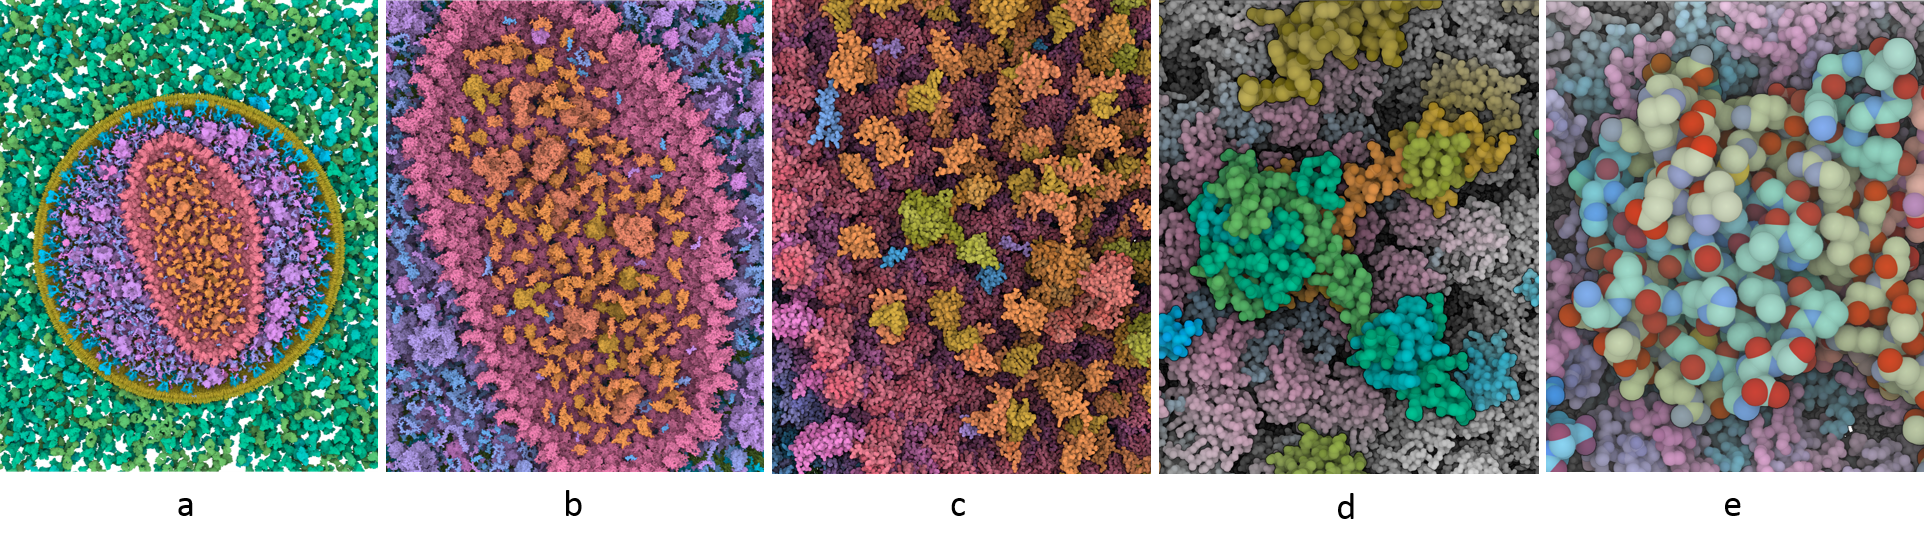
\includegraphics[width=1\linewidth]{Figures/teaser_new}
	\caption{Multi-scale visualization of the HIV virus in real-time, using cellVIEW~\cite{muzic2015cellview} for rendering, together with the presented technique "Chameleon" for dynamic color coding of protein and atom properties.
		The series of vignettes represent, from left to right, a zooming operation from the entire virus down to single atoms.
		Along the way, we modulate the colors to provide relevant information based on the current zoom level.
		(a) At the highest zoom level the orange proteins located inside the capsid are hardly distinguishable, as surrounding compartments which contain more various protein types (green, and purple) are prioritized on the color palette. 
		(b) As we zoom in on the capsid proteins, other compartments become less visible, which allows the capsid protein ensemble to occupy more space in the color palette.
		(c) As we continue zooming, we reveal the domains of the protein by shifting the hue value progressively. Simultaneously, we also shift the luminance to show the presence of underlying structures in the next levels.
		(d) The secondary structures are differentiated by hue, and the atom types by luminance, analogous to the previous levels.
		At the same time we progressively desaturate the context proteins to reduce the number of colors and improve clarity.
		(e) The atom colors are progressively shown as we reach the final zoom level.}
		
	\label{teaserImage}
}

%% Uncomment below to disable the manuscript note
\renewcommand{\manuscriptnotetxt}{}

%% Copyright space is enabled by default as required by guidelines.
%% It is disabled by the 'review' option or via the following command:
% \nocopyrightspace

%%%%%%%%%%%%%%%%%%%%%%%%%%%%%%%%%%%%%%%%%%%%%%%%%%%%%%%%%%%%%%%%
%%%%%%%%%%%%%%%%%%%%%% START OF THE PAPER %%%%%%%%%%%%%%%%%%%%%%
%%%%%%%%%%%%%%%%%%%%%%%%%%%%%%%%%%%%%%%%%%%%%%%%%%%%%%%%%%%%%%%%%

\begin{document}
	
	%% The ``\maketitle'' command must be the first command after the
	%% ``\begin{document}'' command. It prepares and prints the title block.
	
	%% the only exception to this rule is the \firstsection command
	\firstsection{Introduction}
	\label{introduction}
	\maketitle
	
	With improving technology, more and more data across all levels---from atomic to compartment---is being gathered on viruses and cells. 
	Improving computing technology makes it possible to display an ever increasing amount of this data at once, up to and beyond an entire human immunodeficiency virus (HIV)~\cite{muzic2015cellview}, with its complete macromolecular composition.
	This allows all levels to be present in a visualization; we can start at the compartment level and zoom in past the proteins, their domains and secondary structures, such as $\alpha$-helices and $\beta$-sheets, all the way to the amino acids and atoms. Visualization of HIV are not only used for research purposes. Illustrative multi-scale visualizations of HIV have also been used to communicate basic properties of the virus to a broader audience, as in Figure~\ref{fig:motivation}, which is the usage scenario we are interested in.
	
	For each described scale, color contrast is used to distinguish elements on that scale. 
	In interactive visualizations, the color assignment is usually static. 
	At best, users can select their preferred color scheme. 
	Unfortunately, single-scale color mapping will lead either to a loss or an excess of information.
	For example, if we apply color mapping to proteins, then proteins are well conveyed, but the distinction of secondary structures or atoms through color is not possible.
	This is impractical for zoomable visualizations, where a fixed color scheme will either lead to information loss due to uniform colours when zooming in, or salt and pepper noise when zooming out.	
	A naive visualization that defines color maps for each level individually and then blends them may at first glance seem sufficient.
	However, several issues can occur.
	First, colors may change significantly between zoom levels.
	This will not only affect understanding how two levels are connected, but also the comprehension if the user is between levels.
	Second, there is a loss of information when transitioning from one level to the next. 
	For example, if a user is looking at two compartments that are next to each other and zooms in where they meet, then the information where one compartment ends and the other starts is lost, as the compartment level color coding is already blended away. 
	This may also cause orientation problems.
	The reason for this orientation loss is the inherent hierarchy of the data.
	An atom belongs to an amino acid, which in turn belongs to a domain of a protein, all the way to the top.	
	Therefore, a visualization of the data must fulfill three requirements. 
	One, structures should be distinguishable.
	Two, the transtion from one level to another must be smooth.
	Three, the inherent hierarchy of the data must be preserved.
	
	There are several possiblities how to fulfill these requirements. 
	Tenneken and de Jonge~\cite{tennekes2014tree} sub-divide the color space hierarchically so that each branch has its own hue.
	As the tree is traversed towards the leaves through the structures of the cell, the hues become subdivided.
	A compartment could be red, the proteins of that compartment different shades of red, and so forth.
	However, this approach scales poorly with respect to color distinguishability. At smaller scales, colors can become indiscriminable.
	Inherent brightness variations due to shading can additionally influence color perception and limit the number of distinguishable colors.
	
	
	
	%It might appear to be a good idea to branch out into luminance and saturation, in addition to hue.
	%However, this means that the tree expands into three different dimensions.
	%This can cause issues when understanding the data.
	%Varying hue, saturation and luminance all at once can easily lead to cognitive overload, as it is difficult to operate in three dimensions at once. 
	%Furthermore, in an illuminated or shaded scene, two objects with the same hue but different luminance that are next to each other might be %misconstrued as just one object, with the varying luminance userstood as changing structure. 
	%As such, there are significant perceptual and cognitive restrictions placed on color coding. 
	
	We propose a semantic zooming method for a multi-scale visualization of a cell or virus-like structure, based on a view-dependent, hierarchical color scheme.
	Starting from the highest hierarchy level, we progressively free up unused color space and redistribute it to visible elements defined by the current zoom level and item visibility.
	In the HIV as show in Figure~\ref{teaserImage}, the user initially sees the different compartments. 
	As the user zooms in, the proteins receive more distinct colors based on which compartment they are in. 
	As compartments and proteins disappear, the colors of the visible proteins are adjusted to enhance discernibility.  
	As the viewer zooms further in, the domains of the proteins will become distinct, then the secondary structures, and eventually even the atoms, whose colors are predefined by convention.
	
	We will present the concept of our hierarchical color palette, implementation details for real-time rendering in a large scene, and results of a user study.
	In Section~\ref{Overview} we explain the basic structure and idea.
	Section~\ref{sec:hue} describes the implementation details of the coloring .
	In Sections~\ref{sec:chroma} and \ref{sec:luminance} we describe additions that support the visualization.
	In Section~\ref{sec:results} we describe the results.
	Section~\ref{sec:study} contains a user study.
	
	%\begin{figure*}
	%	\centering
	%	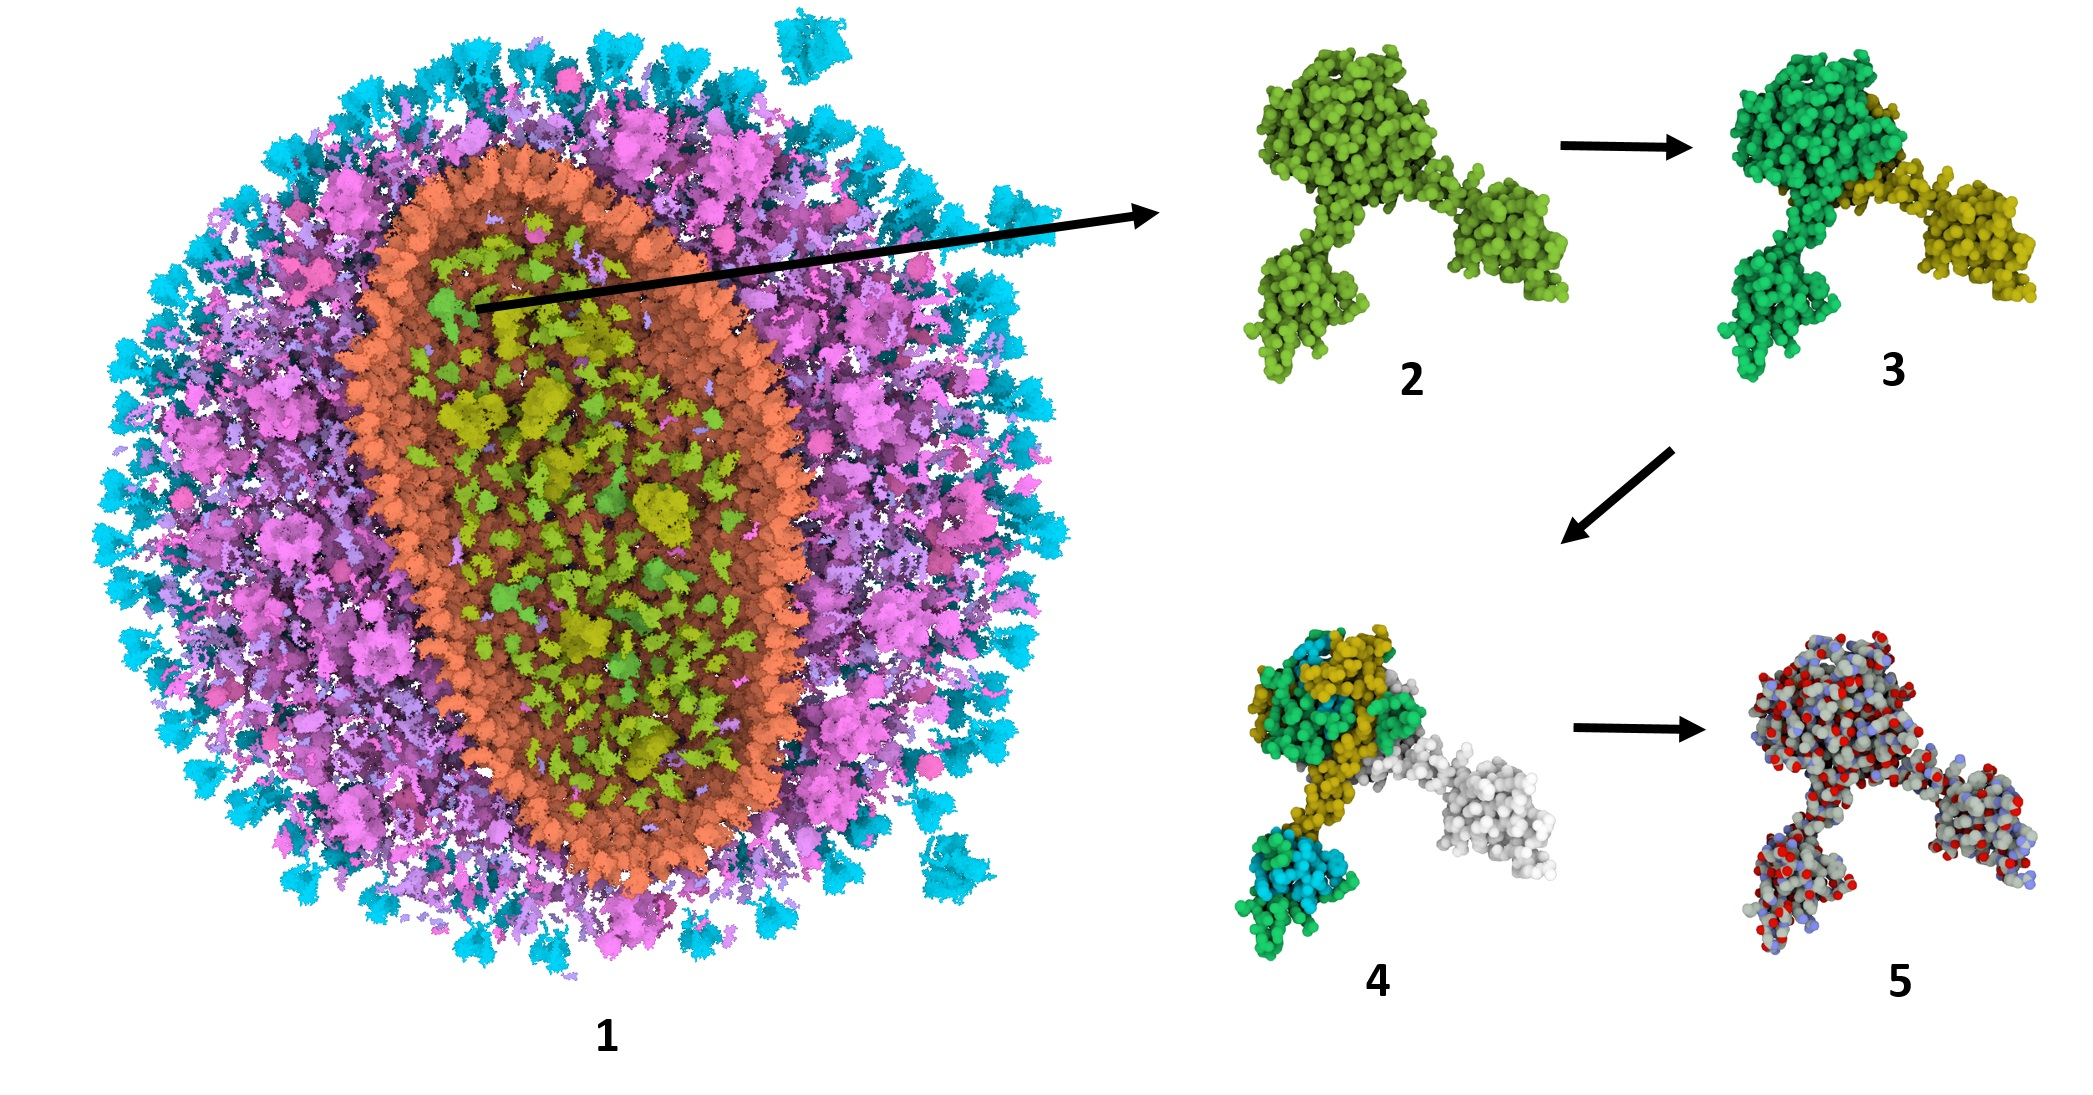
\includegraphics[width=1\linewidth]{Figures/Picture2_}
	%	\caption{Multi-scale visualization of HIV. (1) Cross-section of the virus, proteins are grouped based-on their compartments, and can be distinguished by their colors. (2) Zoom-in on the 1EX4 protein (3) The two domains of the protein are shown. (4) The secondary structures are show for first domain: yellow is for the helices, blue is for the sheets, and green is for the remaining atoms, (5) CPK color coding based on the atom type (blue is for Nitrogen, red is for Oxygen, grey is for Carbon)}
	%	\label{fig:Picture2}
	%\end{figure*}
	
	
	
	%One realm in which this system can be supported in is color. 
	%Color has been consistently and effectively used to seperate objects and sections from each other, and can also be used to display information about the object at the same time. 
	%Therefore, it would be advantageous to use these benefits in such a system. 
	%However, there are significant challenges in doing so. 
	%First, there are not that many easily distinguishable hues. 
	%For example, with constant luminance and chroma, the just noticeable distance - the distance between two colors where the a human can distinguish them - is equal to N degrees, based on a distance of 2.3~\cite{mahy1994evaluation}. 
	%However, this is of course not enough to be easily distinguishable. If 10 times the just noticeable distance were used, we would only have N colors. 
	%Furthermore, if we subdivde the colors when zooming in, similar to a tree, then the discriminability becomes worse with each leve. 
	%Certainly, it is possible to branch out into saturation and luminance as well. 
	%However, varying hue, saturation and luminance all at once can easily lead to cognitive overload, as it is difficult to operate in three dimensions at once. 
	%Lastly, in an illuminated or shaded scene, two objects with the same hue but different luminance that are next to each other might be misconstrued as just one object, with the luminance being used to indicate structure. 
	%As such, there are significant perceptual and cognitive restrictions placed on color coding. 
	
	
	\begin{figure}
		\centering
		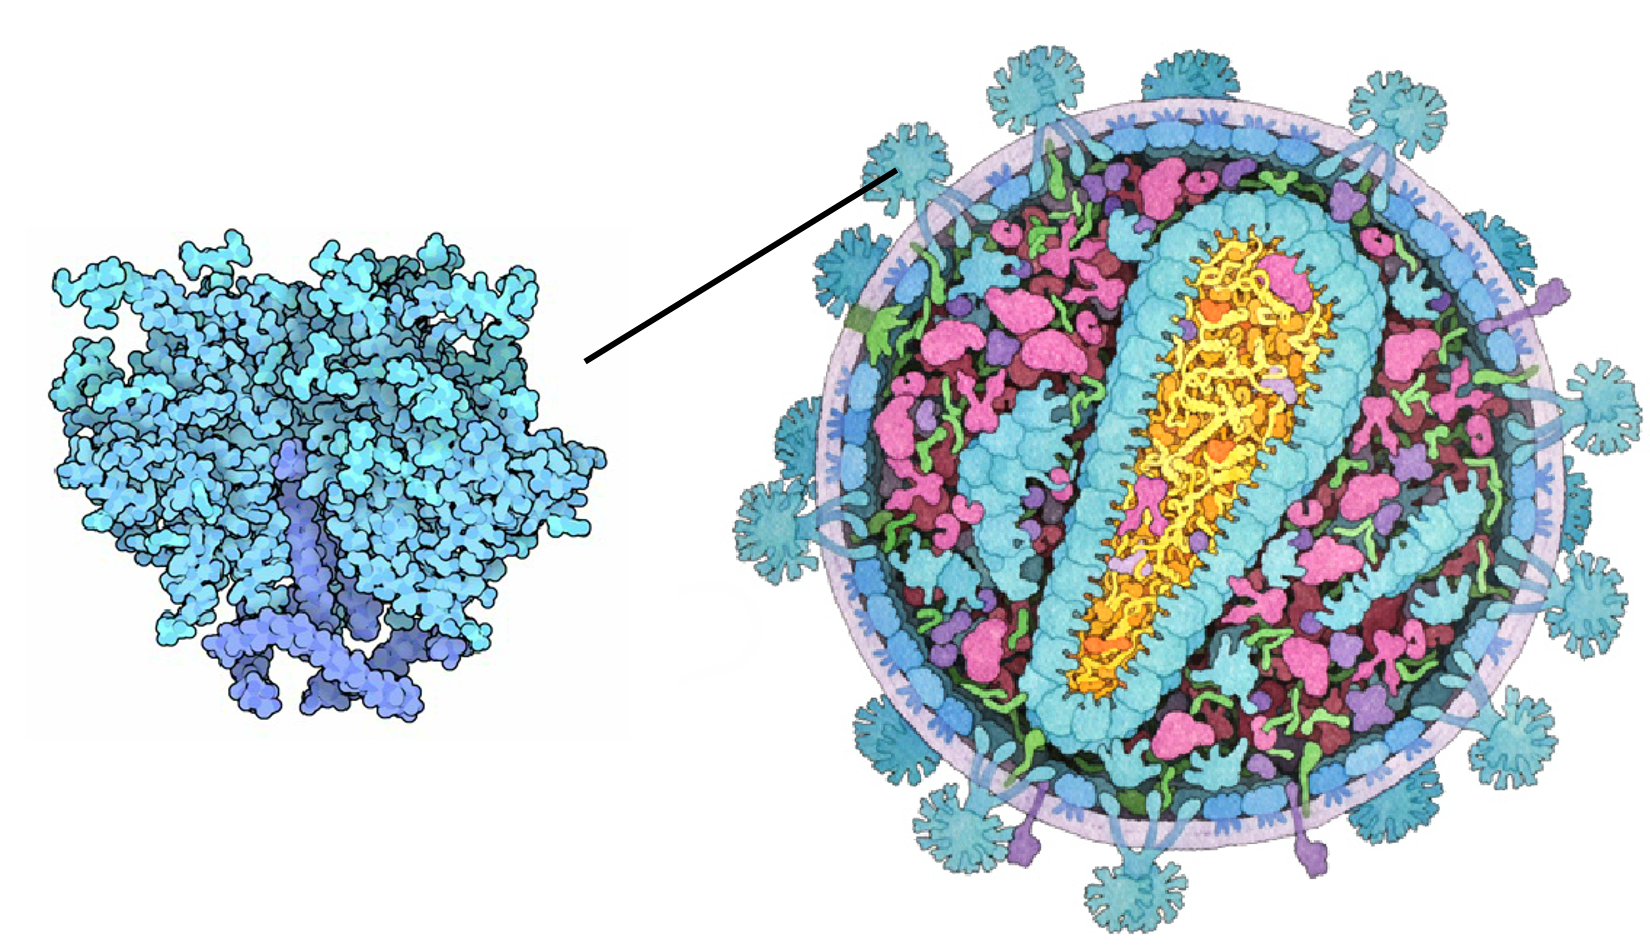
\includegraphics[width=1\linewidth]{Figures/motivation}
		\caption{Motivation: Multi-scale Illustration of the HIV virus from David Goodsell. 
			The left part shows a close up on the protein which is indicated on the right part via the black line.
			In the close-up illustration the illustrator used several shades of blue to distinguish between the different parts of the proteins which are not distinguishable in the wide view on the right side.
			Differentiation is also made between carbon atoms and the remaining ones by shifting the luminance slightly.}
		\label{fig:motivation}
	\end{figure}
	
	
	
	%from here old \newline
	%Biological organisms can be viewed on different scales. 
	%For example, the human body consists of organs, cells, proteins and molecules. As more detailed data is becoming available across all levels, it is possible to combine visualizations of multiple scale levels into a single integrated visual environment. 
	%This poses new challenges for visualization experts, including seamlessly adapting the levels of detail of structural representations for real-time rendering, .... (experts, please address the challenges).
	%
	%A challenge which has not been addressed so far is color-coding. Consider, for instance, the human immunodeficiency virus (HIV).
	%To understand its viral lifecycle, researchers are investigating the shape of its compartments, the role of the individual proteins in viral replication, the secondary structures, as well as structural properties of binding sites on the atomic level. 
	%Traditionally, researchers use dedicated visual representations for each level of scale, and illustrators provide hand-crafted visualizations to communicate new findings to the general public. 
	%Each of these scale levels uses a distinct color coding so that observers are able to distinguish and identify the structures. Can we show existing examples here? 
	%When integrating multiple scales into a single zoomable visualization, it is therefore necessary to not only provide a seamless structural zooming, but also a color-coding mechanism that takes the current level of detail into account. 
	%While successively providing more levels of detail of the structures when zooming in, we are severely limited in the number of available colors due to perceptual constraints and limitations of the monitor hardware. 
	%
	%We propose a semantic zooming method for visualizing color-coded a virusmulti-scale visualization based on a view- dependent hierarchical color-scheme. 
	%Starting from the lowest zoom-level, we iteratively split up the available color space to the number of necessary colors defined by the current zoom level and item visibility.
	% Our method thereby trades discriminability of individual elements against temporal coherence. 
	%In the HIV example (refer to teaser image), the user initially sees the different compartments. 
	%As the user zooms in, the proteins receive more distinct colors based on which compartment they are in. As compartments and proteins disappear, the colors of the visible proteins are adjusted to enhance discernibility.  
	%As the viewer zooms further in, the domains of the proteins will become distinct, and eventually even the atoms, whose colors are predefined by convention. 
	
	\section{Related Work}
	While there has been intense research on color mapping in visualization in the past, there have been only very few works related to multiscale visualization.
	We divide the related work in two sections. In the first section we cover previous work about appropriate usage of colors in visualization, and their perceptual impact. 
	In the second section we cover related work about large scale molecular rendering, to which we build our technique upon.
		
	\subsection{Colors in Visualization}
	The selection of  a color map for data depends heavily on the visualization goal. 
	Not only clear visibility, but also harmonious and appealing colors can be important~\cite{ihaka2003colour}, as well as the assignment and mixing of colors~\cite{wang2008color}. 
	There are many points to consider, and as a result guidelines have been published on how to decide which color scheme is the most appropriate~\cite{bergman1995rule}, \cite{healey1996choosing}. There have also been guides aimed at two dimensional color maps, such as \cite{bernard2015survey} and the software ColorMap-Explorer by Steiger et al.~\cite{steiger2015explorative}.	
	Furthermore, several tools have been developed to assist users select appropriate color maps, such as Colorbrewer~\cite{harrower2003colorbrewer}, including color maps for clusters of data, such as "i want hue"~\cite{iwanthue} and XCluSim~\cite{l2015xclusim}. 	
	Such clustering can, however, cause perceptual issues, either due to the large number of clusters or their layout. 
	Particular care needs to be taken when dealing with higher dimensional data~\cite{mittelstiidt2014revisiting}, so the distances between the clusters do not become distorted. 
	Furthermore, in cases such as coloring maps, visually dominant structures may visually suppress small groups or areas~\cite{lee2013perceptually}.
	Visualization of information such as can be found on maps can lead to small areas being next to much larger ones. 
	In this case, it may be difficult to spot the small areas, and lowering the saturation of the larger areas allows the small ones to stand out more.
	Recognition may also be affected by contrast effects which may need to be dealt with~\cite{mittelstadt2014methods}. 
	
	XCluSim’s uses a tree-based method~\cite{tennekes2014tree} that attempts to overcome these issues in the case of hierarchical structures. 
	The tree method uses HCL space (a cylindrical coordinate version of CIELab with Hue , Chroma (Saturation), and Luminance) and gives each cluster a different hue. 
	The root of the tree has no saturation, i.e. grey, and the hue is divided up into different wedges, one for each branch, with some space cut out between branches, in order for there to be a jump in color from one wedge to another. 
	As the tree spreads out, the saturation of the nodes increases, and each level gets its own smaller wedge. 
	Essentially, each level has its own hue circle with a defined chroma. 
	However, it was designed for static visualizations, where all colors are visible at the same time. Therefore, the number of possible colors is severely limited, leading to discriminability problems.
	In contrast, our method allows for dynamic increasing and decreasing of wedge angles based on visibility and depth, allowing for overlap to occur at the lower levels. 
	If some of our branches' nodes are not visible, then the wedge will shrink, allowing neighbouring branches to expand. 
	This assists color discernment by the user when looking at the objects of a subset of the branches.
	
	
	%Color maps are used often in visualization. Their structure depends heavily on the application, as has been shown in [Colour for Presentation Graphics], [Color Design for Illustrative Visualization]. Several tools have been developed 
	%
	%Color maps are used often in visualization. 
	%Their structure depends heavily on the application, as has been shown in [Colour for Presentation Graphics], [Color Design for Illustrative Visualization], 
	%
	%A Rule-based Tool for Assisting Colormap Selection, http://ultra.sdk.free.fr/docs/Image/Colors/ARule-basedToolfo0AssistingColormapSelection.htm], [Choosing Effective Colours for Data Visualization], 
	%[a survey and task-based quality assessment of static 2d colormaps], [explorative analysis of 2d color maps]. 
	%Several tools have been developed to assist users select appropriate color maps, such as colorbrewer, or iwanthue, [http://tools.medialab.sciences-po.fr/iwanthue/] and XCluSim, which are aimed at generating colors for clusters of data. 
	%However, when dealing with numerous clusters, special attention must be paid to the perceptual qualities of the color map
	
	
	%\subsection{multiscale view}
	%Sometimes hierarchical data can also be viewed on multiple levels at once, for example a protein can be viewed on the overall structure as well as on the atomic structure~\cite{kauker2013rendering}. 
	%Alternatively, distortions of the object or different rendering levels in different areas of the camera may be used. 
	%For example, in~\cite{hsu2011rendering} the area in the center of the camera is rendered as closer in. 
	%This is achieved through using non-linearly bent camera rays and multiple cameras. 
	%Parts of the object can also be distorted, for example by widgets such as in~\cite{sudarsanam2008non}, where local areas are distorted using non-linear perspectives. 
	%Alternatively, the user might want to zoom into a structure. An example of this is~\cite{artignan2009multiscale} in which a large hierarchical graph is visualized.
	%The graph has a large depth, and to investigate certain nodes the user must zoom in. During this, the node expands and changes color while its children become exposed. 
	%This is recursively applied down the branch, allowing for an arbitrarily deep descent.
		
	\subsection{Multi-Scale Molecular Visualization}
	
	The development of new modelling techniques for three dimensional molecular structures led to a rapid increase in size of the studied datasets.
	To keep up with the progress, new visualization methods were specifically developed to address this challenge.
	Lampe et al.~\cite{lampe2007two} pioneered real-time rendering of large-scale atomic data on consumer level hardware. 
	They extended the fast billboard-based approach introduced by QuteMol \cite{tarini2006ambient}, by rendering the structures per residues rather than per atom, thus reducing the memory bandwidth usage and the GPU driver overhead. 
	Lindow et al. \cite{lindow2012interactive} followed-up by using  instanced rendering to draw entire structures instead.
	For each molecule type, they generate a 3D grid of the atoms which is stored on the GPU, and then ray-casted upon rendering.
	Falk et al. \cite{falk2013atomistic} further refined the method with improved depth culling and hierarchical ray casting to achieve faster rendering performance for even larger scenes.\\
	
	Parulek et al.~\cite{parulek2014continuous} introduced seamless transitions between different levels of coarseness for the representation of the molecular surface based on the distance from the camera.
	The goal was not only to reduce the computation cost, but also to utilize the shape as a means to reduce high-level details and noise when observing the structure in its entirety.
	Their technique uses real-time ray-tracing and offers high quality surface details, but it does not scale well in terms of performance when compared to atom-based rendering methods.
	A novel approach, for real-time rendering of structures with up to tens of billion atoms, was later on introduced by Le Muzic et al.~\cite{le2014illustrative}. 
	Their approach, also based on level-of-detail, uses tessellation shaders to switch between different degrees of coarseness for the molecular structures, on-the-fly and upon the rendering operation.
	The entire scene is thus rendered efficiently in a single draw call, approaching zero GPU-driver overhead. 
	As a follow up, they developed and released cellVIEW \cite{muzic2015cellview}, a tool designed for rendering large-scale molecular scenes, which was implemented with Unity3D, a popular 3D engine.
	cellVIEW was primarily developed to showcase large molecular structures generated with cellPACK \cite{johnson2015cellpack}, a tool developed to procedurally generate accurate and multi-scale models of entire viruses and cells.\\
	
	The Chameleon is built upon cellVIEW, and is an attempt to improve understanding during exploration of multi-scale molecular scenes generated with cellPACK.
	cellVIEW leverages GPU computing and parallel programming to provide a fluid user experience, Chameleon was developed with the same programming paradigm.
	
%	\begin{figure}[t]
%		\centering
%		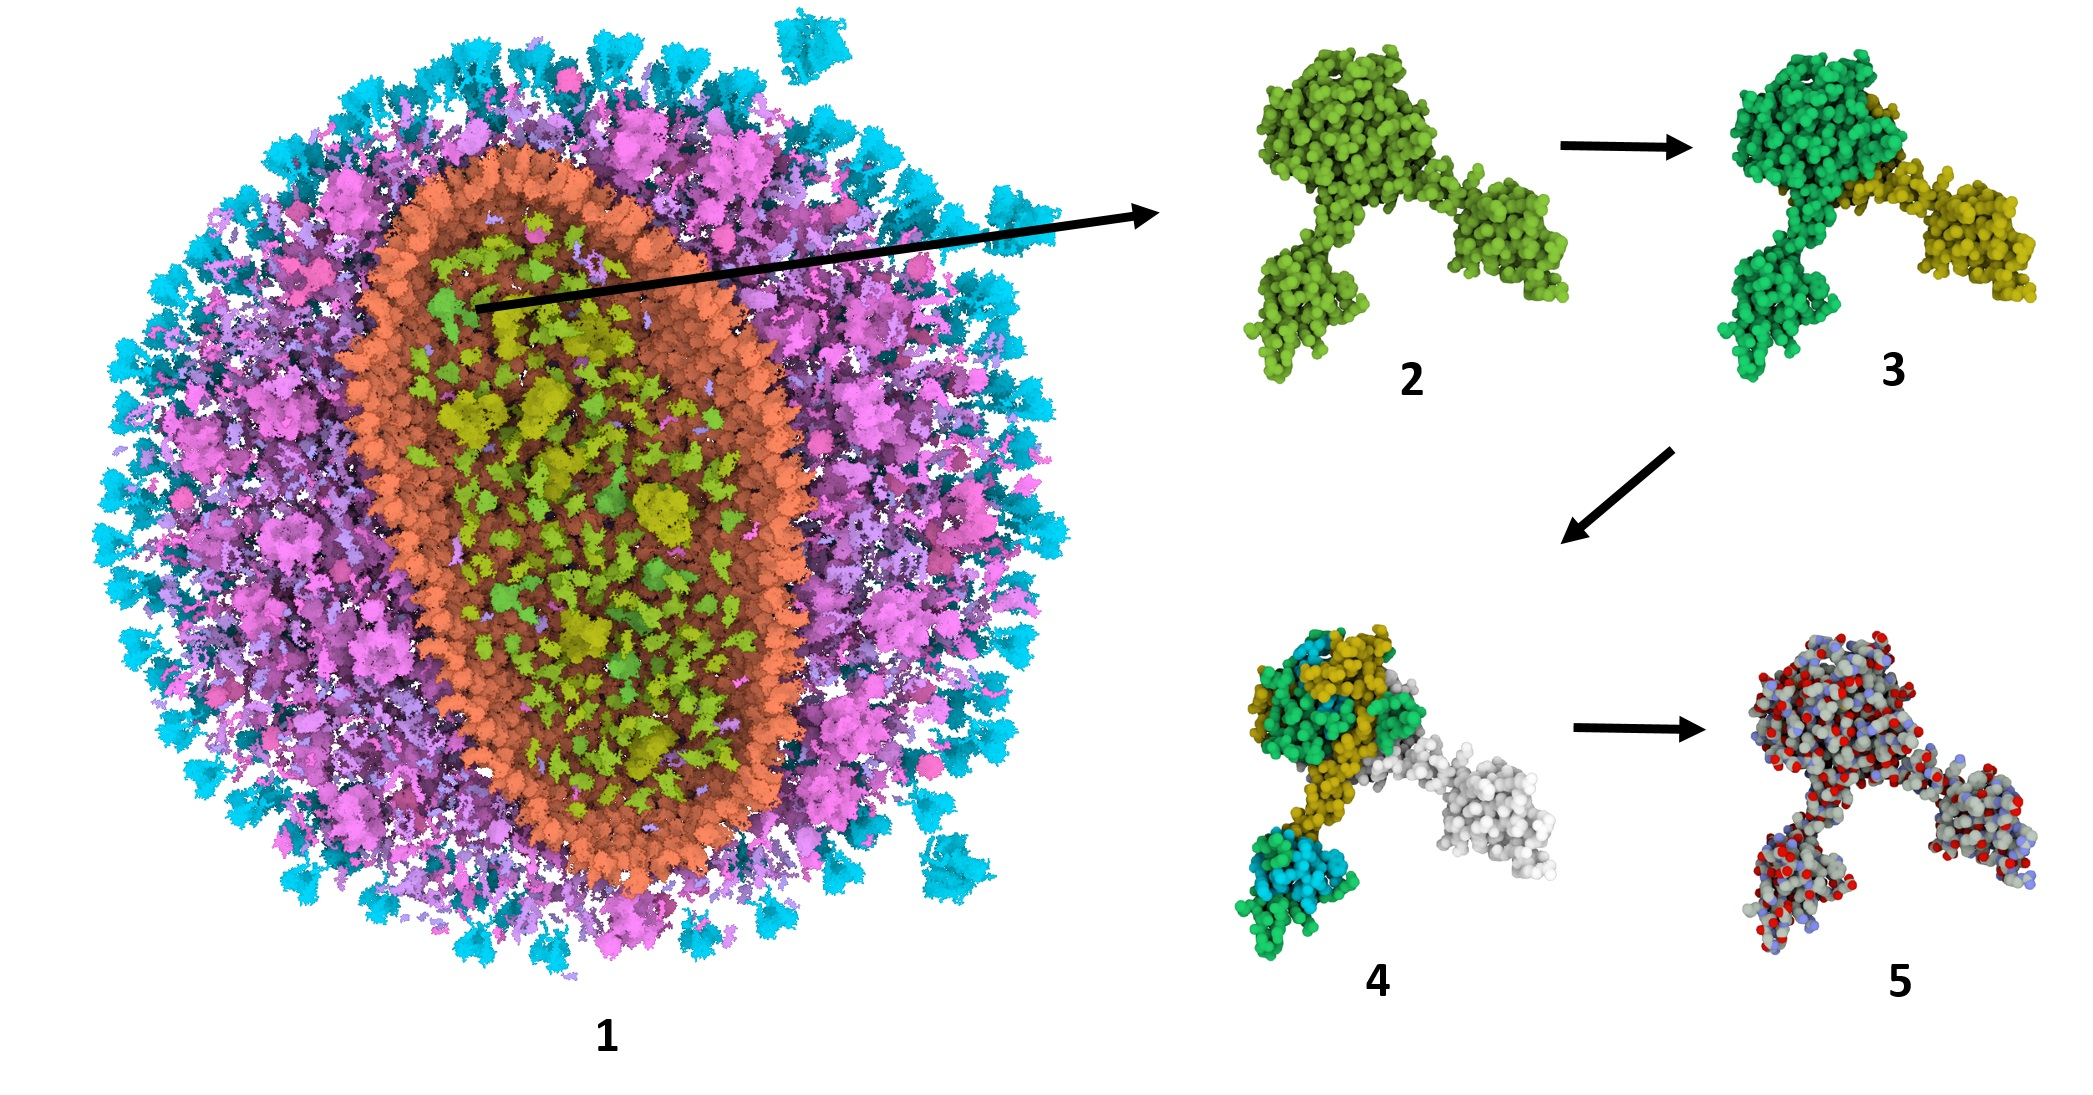
\includegraphics[width=1\linewidth]{Figures/Picture2_.jpg}
%		\caption{Multi-scale visualization of HIV. (1) Cross-section of the virus, proteins are grouped based-on their compartments, and can be distinguished by their colors. (2) Zoom-in on the 1EX4 protein (3) The two domains of the protein are shown. (4) The secondary structures are show for first domain: yellow is for the helices, blue is for the sheets, and green is for the remaining atoms, (5) CPK color coding based on the atom type (blue is for Nitrogen, red is for Oxygen, grey is for Carbon)}
%		\label{fig:Picture2}
%	\end{figure}
%	


	

		
	\section{Chameleon Overview}
	\label{Overview}
	
	Mesoscale datasets feature many relevant properties which are present at different scale levels.
	The molecular properties that we provide are, from the largest to the smallest scale level: compartment (which we refer to as protein group), protein type, protein domain, secondary structure and atom type.
	According to domain experts, these are the most relevant properties in visual analysis of three dimensional molecular structures.
	%We opted for these properties because, according to domain experts, they are the most relevant properties in visual analysis of three dimensional molecular structures.
	%This information is internally declared and accessible for each single rendered atom, which allows us to perform dynamic coloring.
	Scientific illustrators are using these properties to modulate the color palette when showing proteins at different levels, as shown in Figure~\ref{fig:motivation}.
	However, this requires to manually set up the color palette for each level, which can be cumbersome when dealing with a multitude of large datasets.
	Our goal is to provide a dynamic coloring mechanism that would automatically assign and display the most relevant information for any given zoom level, thereby fulfilling the requirements stated in the introduction: 
		
	\begin{enumerate}
		\item On each zoom level, associated main structures (i.e., those structures that result in the best visibility in terms of screen size) should be clearly discriminable from each other. 
		\item When navigating, the transitions between the zoom levels should be smooth to avoid abrupt appearance changes of visualization or orientation loss. 
		\item The inherent hierarchy of the structures should be reflected in the color coding. 
		\item The visualization should be aesthetically pleasing to engage a broad audience. 
	\end{enumerate}
	
	We manipulate all three color components to fulfill these requirements: 
	We use the \textbf{hue} to distinguish between structures at the respective zoom levels, as described in Section \ref{sec:hue}. 
	The \textbf{chroma} is used to increase color discriminability for elements in the focus against the context (Section \ref{sec:chroma}). 
	Finally, we indicate structures from lower hierarchy in the \textbf{luminance} channel to mimic illustrator techniques (Section \ref{sec:luminance}). 
	We describe how we dynamically adapt the hues as the user navigates the scene to ensure color discriminability even in a scene with dozens of different entities (Section \ref{sec:dynamic}), and how hues are sub-divided hierarchically as the user zooms further into the scene (Section \ref{sec:hierarchy}). 
	Finally, we demonstrate the effectiveness of our technique in a user study with domain experts from the field of molecular biology (Section \ref{sec:study}). 
	
	
	
	%This information should also be coherent between levels.
	%To provide smooth and logical transitions across levels, we use a hierarchical color coding approach inspired by a tree-based coloring method~\cite{tennekes2014tree}.
	%Based on perceptual reasoning, clarified in the introduction, we use isoluminant colors, and we choose to only vary the hue channel to generate the color palette. 
	%
	%On the first level of the hierarchy, we first assign portions of the hue circle to each group of protein types.
	%Protein types of a given group are then given a unique hue value on the corresponding arc, as shown in Figure \ref{fig:coloroverview}.
	%In the initial state, the size of the hue arcs is set according to the number of protein types contained in each group. 
	%Spacing between hue values of neighbour protein types of the same group is proportional to the number of type per group and the size of the arc. 
	%
	%Due to the large difference in terms of size between groups and proteins, it is very likely that several compartments will be less or no longer visible as we zooming-in on a single protein. 
	%Based on this principle we update the color palette on-the-fly using the visibility information which we extract from the previously rendered frame.
	%For each protein type, we compute the percentage of visible elements, as well as the screen coverage in pixels for displayed proteins.
	%We sum up those properties for all the protein types of a group to deduce a weighting coefficient which is then used to scale the size of the hue arcs of the groups as shown in Figure~\ref{fig:coloroverview}.
	%
	%When zooming further in, we progressively start to reveal colors of the underlying protein properties, such as the chains, or secondary structures.
	%For coloring the subsequent levels, we sample hue values around the hue of their parent as shown in Figure~\ref{fig:coloroverview}.
	%We use pre-defined camera distance thresholds to determine when to transit to the next level.
	%To ensure a smooth transition, the hue distance between the parent and the children is progressively scaled until reaching a pre-determined offset value.
	%%In the case of protein types, the coloring mechanism allows to enlarge the size of the hue arcs while ensuring no overlap between neighbooring groups. 
	%%However, when displaying other properties it would be more challenging to reuse the same principle, because of ** TODO REASONS **.
	%To ensure a minimum degree of overlapping hue ranges between two neighbours, we use a focus + context to reduce occurence of recurrent colors in the background.
	%
	%Atoms constitute the final level of our hierarchy.
	%In molecular visualization this information is commonly associated with predefined colors also called CPK coloring.
	%To transit to this final level we perform linear color interpolation in RGB space, between the color from the previous level (secondary structures) and final atom color.
	%The coefficient of interpolation is defined according to the camera distance and pre-defined distance values *** MANU'S MAGIC COLOR INTERPOLATION HERE ? ***.
	%
	%\textbf{. With a static hierarchical color coding approach, the hue arcs are predefined on the highest level, and multiple colors are then generated for the lower levels by manipulating channels like chroma luminance} \\
	%
	%\textbf{. The strictly static approach has two limitations:}
	%
	%\textbf{. It uses luminance variation to generate distinct colors, which is not preferable to use with a lit 3D environment} \\
	%
	%\textbf{. Hue arcs are statically defined, therefore, in case the entire wheel is occupied, colors generated inside the wedge do not have an optimum degree of discriminability.  } \\
	%
	%\textbf{. Indeed, HUE is such a stronger cue to differentiate between types** add better justification **}
	%
	%\textbf{. Therefore we suggest a method to define color coding hierarchically, where the initial hue value would no longer be statically defined }. \\
	
	%\textbf{. The principle is to use the view information to enlarge to interact with the size of the hue arcs on the highest zoom level.} \\
	%
	%\textbf{. A naive approach would be to simply increase the hue arcs as the camera gets closer to an element and to interpolate between levels based on the distance. }
	%
	%\textbf{. However, by increasing the arc lengths arbitrarily we will inevitably run into a case where two consequent segments would overlap } \\
	%
	%\textbf{. This shall be avoided when possible in order to ensure a maximum level of clarity } \\
	%
	%
	%\textbf{. We address this problem differently based on the zooming level, via two different approaches} \\
	%
	%\textbf{. Indeed, in mesoscale datasets, the multiple semantic levels from entire viruses or cells, down to single atoms, are not evenly spaced.} \\
	%
	%\textbf{ . **TODO** ruler figure with all the scales}
	%
	%
	%\textbf{By observing the scale we realize that the size difference between levels beneath the protein levels is much lower than the levels above.} \\
	
	
	%\section{Details Info Dump}
	%
	%full sentences are commented in the tex
	%\textbf{. Molecules have multi-scale properties which can all be characterized by color } \\
	%
	%%.The scenes that we are displaying represent meso-scale biological structures and comprise a large number of molecules (proteins or lipids).
	%%.Each protein carry essential properties that is used to convey a different information for each single scale (TODO: Do a figure to explain).
	%%.Each of these properties can be visualized and highlighted using a specific color coding.
	%
	%\textbf{. Molecules have Bottom-Up properties, type and group} \\
	%
	%%. Molecules can be of different species or type, which characterize their structure.
	%%. A group of molecules with similar structures is referred as instances of type X.
	%%. Types are also categorized in groups, based on their location or function. 
	%
	%\textbf{. Molecules have Top-Down properties, domain, secondary structures, and atom type} \\
	%
	%%. Each molecule comprise a set of atomic particles.
	%%. Atoms have different types, C, H, O, N,...
	%%. Atoms are assembled in groups to form the amino-acids.
	%%. Amino-acids are chained and form segments of amino-acids that are characterized by their shape such helices and sheets, this is called the secondary structure.
	%%. The secondary structures are grouped together and divide the proteins in different domains.
	%
	%\textbf{. BOTTOM-UP PROPERTIES} \\
	%
	%\textbf{. We use hierarchical color assignments for Bottom-Up properties (we defined wedges in the color wheel for the groups and types inside a group are assigned a color in the corresponding wedge )} \\
	%
	%%. We decide to chose iso-luminant colors (for aesthetic reasons).
	%%. We first assign a wedge of the color-wheel for each group.
	%%. In the initial state, the size of the wedge is proportional to the size of the group in terms of protein types.
	%%. The colors of the protein are defined accordingly to the color of their group (hierarchical).
	%%. Only the hue differs between different types of molecules
	%%. Inside a wedge each protein type of a group is assigned to a portion of the wedge with equal spacing between two protein types.
	%%. Should a wedge be enlarged or shrunken, the color assignment is set relatively to the size of wedge.
	%
	%\textbf{. Static tree color maps offers limited discrimination for a large number of colors because it uses other properties to vary colors inside a wedge, HUE IS A MUCH STRONGER CUE} \\
	%
	%%.The hue circle is limited (360), therefore with several groups comprising tens of individual types we will quickly run out of colors.
	%%.In the tree-color paper they solve this problem by generating more colors for each wedge using the additional channels (chroma \& luminance).
	%%. This approach has a poor potential for discrimination between different properties since inside a predefined inside a wege colors will still remain rather similar. 
	%
	%\textbf{. NAIVE APPROACH: Grow the size of color wedges dynamically when zooming in to vary the hue of the colors inside a wedge} \\
	%
	%%. Rather than using different channels like luminance and chroma we want to keep discriminating colors with HUE because it is such a strong cue.
	%%. In order to keep using the hue to discriminate between colors the size of the wedges must be scale according to the zooming distance.
	%%. However as the wedges grow their is no mechanism that would prevent two neighbour wedges to overlap which could results in misleading coloring choice.
	%
	%\textbf{. Wedges may overlap, solution is to use visibility information to control the scaling of the wedges} \\
	%
	%%. Rather than scaling the wedges according to the zooming distance we suggest to grow or shrink the wedges according to what is currently visible in the current viewport.
	%%. For example, if all molecule groups are equally visible, the size of their wedges will be proportional to the size of the groups in terms of protein species.
	%%. If a protein group is partially visible or not-visible at all, the corresponding wedge will be scaled accordingly, thus freeing space in the color wheel for other wedges to grown
	%%. [Make figure to show example]
	%
	%\textbf{. Read Visibility Information must be read form the current viewport} \\
	%
	%%.We analyse visibility information from the rendered frame to check which molecules types are actually currently visible.
	%%.The visibility information we use is screen coverage and number of visible instances.
	%%.The number of visible protein can be low, while few molecule can have a large screen pixels coverage if located close to the camera.
	%%.Similarly the screen coverage can be low while a large number of molecules may still be visible, if camera is looking a the scene from far away.
	%
	%\textbf{. Use Visibility Information to control the sizes and the layout of wedges, via force fields} \\
	%
	%%. Once we have the visibility information for each species we evaluate the weight of the species group for scaling the wedge.
	%%. We use a force based layout to arrange the wedges along the color wheel.
	%%. Each wedge comprise a centroid that can move either left of right, in one dimension.
	%%%. The position is then mapped from 1D to a 2D circle for debugging.
	%%. Each wedge acts as a circular force field centred around the centroid and which pushed the other wedges away.
	%%. The radius to force field is proportional to the size of the group, the number of visible instances, and the percentage of pixels that are occupied by instances of the group.
	%%. The radius of the force field is computed as follows: write formula here.
	%%. The integration of the forces is computed as follows: write integration formula here.
	%%. To make sure that wedge centroids are not pushed away too much from their original location and are shifting in color too much we also apply attraction forces from the centroids to their original location
	%
	%
	%\textbf{. TOP-DOWN PROPERTIES} \\
	%
	%\textbf{. To transition between two down properties we rely mostly on the camera distance rather than the visibility information} \\
	%
	%\textbf{. We use HUE again as a cue to discriminate between sub-domains of a protein} \\
	%
	%\textbf{. We chose HUE values for the chains that are located in the vicinity of the Protein HUE value} \\
	%
	%\textbf{. We perform smooth transition between protein HUE and terminal HUE chain as the viewer zoom-in} \\
	%
	%\textbf{. When focusing on proteins to observe the chains, the chain HUE values of neighbouring or likely to cross/overlap those of the focus} \\
	%
	%\textbf{. We came up with the idea to prioritize the display of chain properties to proteins with a high screen coverage} \\
	%
	%\textbf{. Additionally when zooming closely to a protein to observe bottom-up properties, we desaturate proteins with low screen coverage to reduce clutter cause by the display of too many top-down property colors for context molecules } \\ 
	%
	%
	%\textbf{At the finest zoom-level we show the atom colours, these colors follow bio-chemical standard and are therefore predifined. } \\
	%
	%\textbf{We perform color smooth color interpolation between the current color of the atoms and their terminal colors. } \\
	%	
	%\textbf{To improve the bla-bla, we use the interpolation technique by Manu which constists of bla-bla-bla} \\
	
	
	\begin{figure}
		\centering
		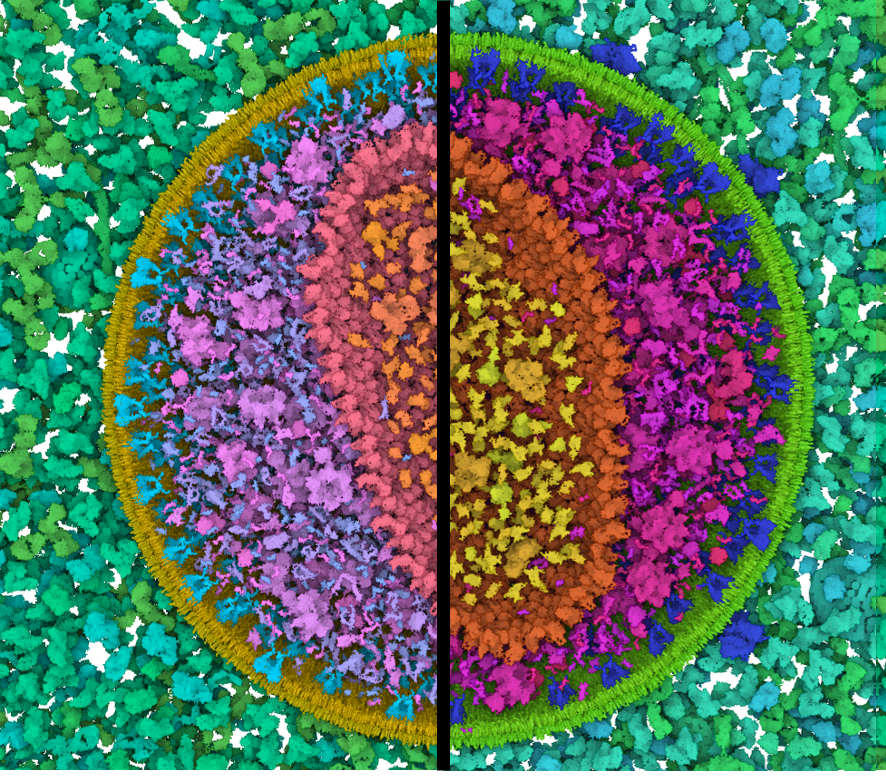
\includegraphics[width=0.75\linewidth]{Figures/hslvshcl}
		\caption{Comparison between two color palettes with varying hues and constant saturation/lightness using HSL (left), and constant chroma/luminance using HCL (right). 
		Unlike HSL, the HCL color space provides true isoluminant colors when varying the hue with constant chroma/luminance values.
		 Mind how the dark blue colors, inside the virus and next to the membrane, make it hard to distinguish individual proteins in a lit environment.}
		\label{fig:hslvshcl}
	\end{figure}
	
		\begin{figure*}[t]
			\centering
			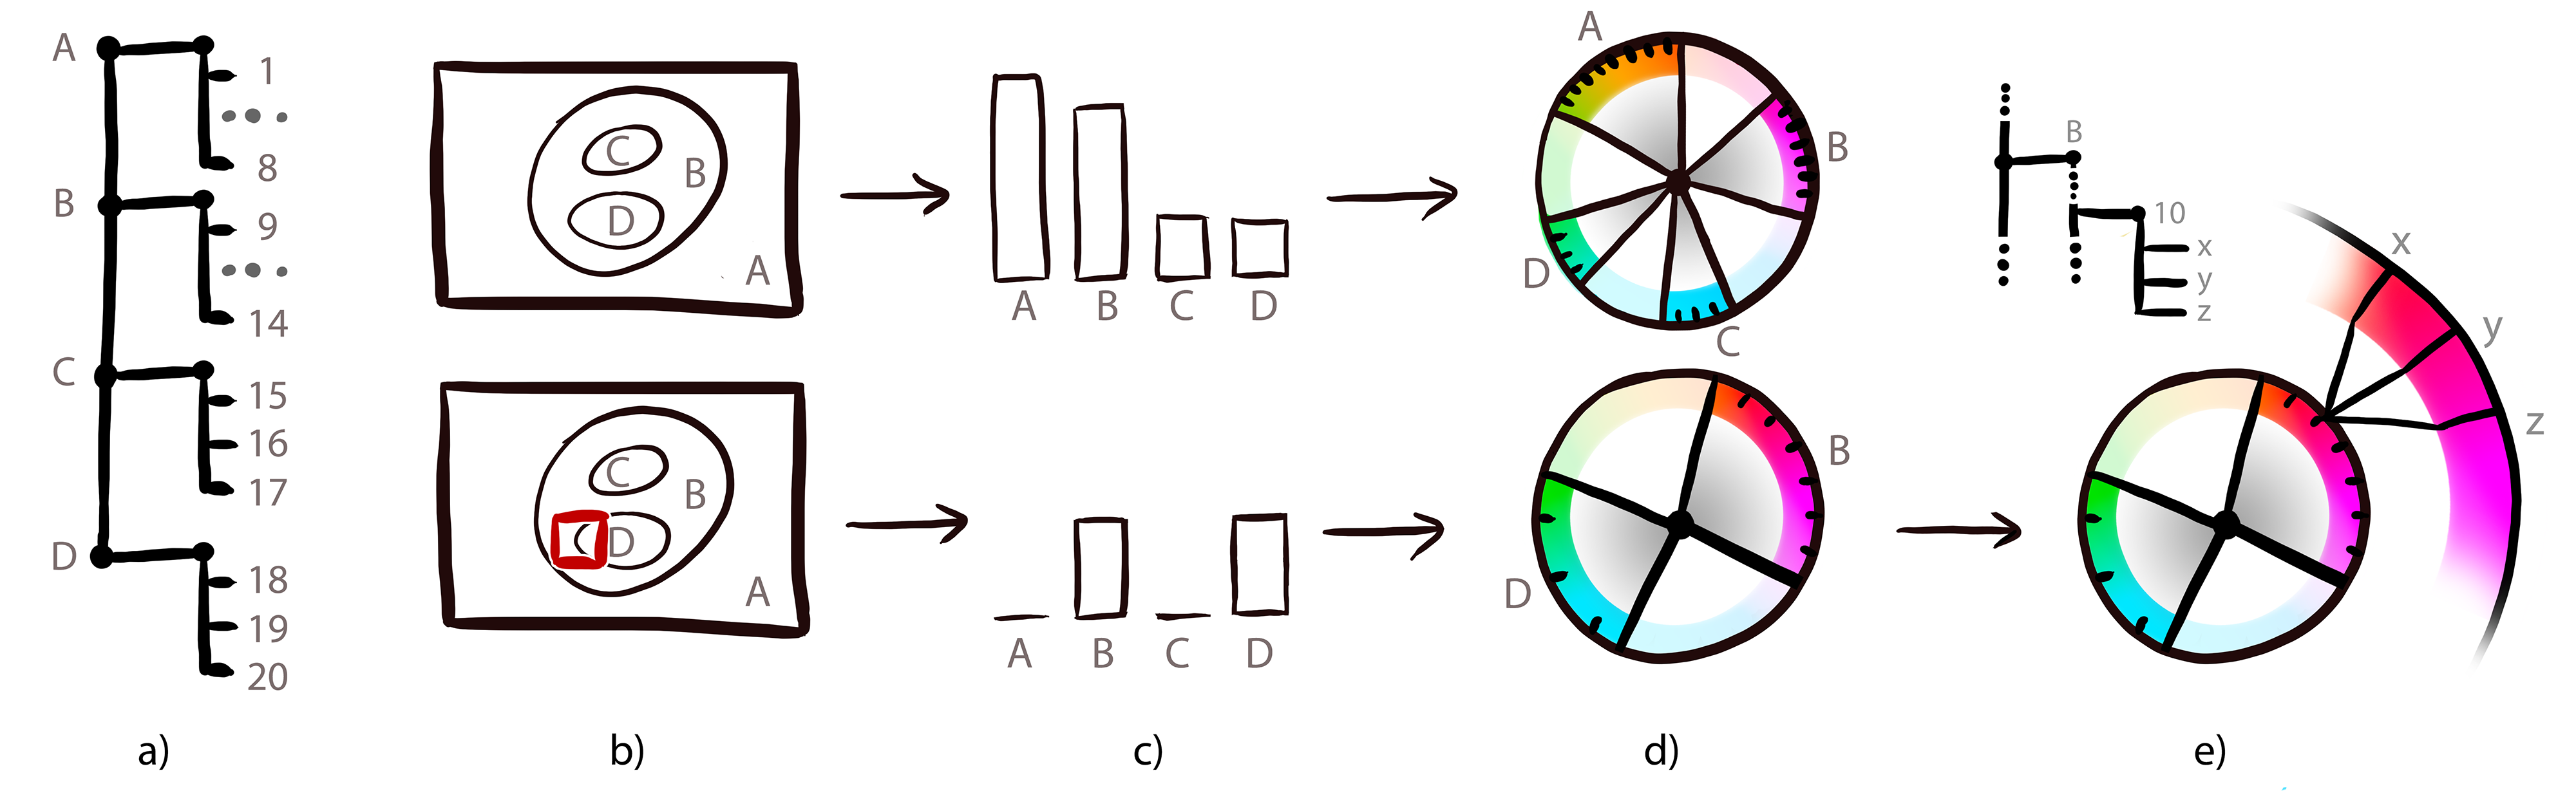
\includegraphics[width=0.95\linewidth]{Figures/coloroverview}
			\caption{Overview of our dynamic and hierarchical hue selection scheme. (a) Shows the first two levels of the hierarchy, in this demonstration case there are four groups of protein types (A,B,C,D) with an overall number of 20 different protein types, (b) Shows the current viewport, wide view on the top and close-up on the bottom, where the red square represents the actually viewport, (c) The visibility information is extracted from the current viewport and analysed, (d) The color palette is updated to include visible elements only, (e) The following levels of the hierarchy (domains only in this case) are revealed as we zoom in on a protein of type 10, which features 3 different domains (x,y,z).}
			\label{fig:coloroverview}
		\end{figure*}
	
	\section{Dynamic Hue Palette}
	\label{sec:hue}
	
	In the highest hierarchy levels (protein and compartment), our task is to find colors for each individual protein type that allow users to discriminate the proteins, but at the same time understand their hierarchical grouping into the compartments. 
	Also, aesthetics are important, as we target our work at interested users from a broader audience. 
	
	Due to aesthetic reasons, we opted to choose only saturated and iso-luminant colors, resulting in a pastel color palette. 
	Figure \ref{fig:hslvshcl} shows a comparison between an iso-luminant and non-iso-luminant color palette for our visualization. This and the use of chroma and luminance described in Section~\ref{Overview} illustrate our design choice. 
	We therefore keep the chroma and luminance constant and color the proteins by hue only. 
	To have better control over color discriminability, we work use CIELab and HCL color palettes, respectively, which are perceptually linear. 
	This means, we can quantify the dissimilarity between colors by their Euclidean distance in the color space. 
	With constant chroma and luminance, hues are selected from a iso-luminant hue ring with uniform chroma. 
	
	To select suitable chroma and luminance values, we investigated which luminance values result in the largest possible hue ring when converting colors from CIELab space back to sRGB. 
	In an offline procedure, we picked eight extreme a and b values with equal distance from the non-chromatic center with a given L value and iteratively moved them towards the center until the resulting CIELab color was lying within the sRGB gamut. 
	The smallest vector magnitude of $\vec{ab}$ thereby defined the radius and chroma for the given luminance, respectively. 
	We found that a luminance of 75 represents a good value, leading to a maximum chroma of 40 (see Figure \ref{fig:hslvshcl}). 
	
	In order to calculate the color of the compartments and their proteins, we can distribute the hues of the hue ring to the different proteins.
	The color of the compartment will then simply be at the center of the proteins that belong to it.
	To distribute hues from the hue ring to the proteins, we sample the hues with respect to four parameters: 1) the number of compartments $n$, 2) the number of protein types $m_i$ within each compartment $1 \leq i \leq n$, 3) the optimal color distance between structures $d$, which will be elaborated below, and 4) the minimum color spacing $s$ between compartments. 
	This corresponds to the top row of (b), (c) and (d) in Figure~\ref{fig:coloroverview}.
	The first parameter defines the number of ``wedges'' that are overlaid on the hue ring. 
	The second parameter controls the relative angular width of the wedges. 
	The third and fourth parameter control the actual angular width of the wedges: 
	Given the chroma $C^*$ (i.e.\, radius) of the hue ring and the optimal Euclidean color distance $d$, the angular distance between neighboring proteins within the same compartment is defined as: 
	\[
	\alpha = arcsin\frac{d}{C^*}. 
	\]
	Empirically, we found that $d$ around 11 delivers results which correspond to around 5 \textit{``just noticeably different''} steps of 2.3 in CIELab color space \cite{lee2013perceptually}, allowing for easy discrimination and pleasing results. 
	Assuming no spacing between compartments (i.e.\, $s=0$), this would result in only 32 distinct colors, which is far below the number of proteins we have in the HIV model. 
	The angular distance  $\alpha$ between proteins will therefore be below the optimal $d$ and defined by 
	
	\[
	\alpha= \frac{360}{\sum_{i} m_i - n \cdot s}. 
	\]
	
	This means, as we zoom out, the colors become very similar and hard to distinguish. However, 
	in the overview zoom level, this effect is actually desirable to avoid salt and pepper noise. 
	As we zoom in, we want increasing discriminability, as defined by parameter $d$. 
	We therefore introduce a dynamic, view-dependent color adaptation approach. 
	
	%\textbf{MWA END: my suggestion is to remove the next paragraph}
	
	

	
	\subsection{View-Dependent Color Adjustment}
	\label{sec:dynamic}
	
	In the initial state, we first generate a color palette assuming that all the compartments are visible.
	As we zoom-in and explore the scene, large parts of the scene may not actually be visible in the current viewport, as is illustrated in the lower row of Figure~\ref{fig:coloroverview}.
	In this configuration the color palette would become underexploited, and could be improved to increase discriminability between proteins that are currently visible. 
	We therefore re-compute and optimize the color palette on-the-fly, as proteins appear and disappear.
	An overview of the mechanism is described in Figure~\ref{fig:coloroverview}.
	
	In order to determine which protein groups occupy unnecessary space in the color palette, we extract the visibility information by analysing the previously rendered frame.
	For each entire group of protein types, we derive a visibility coefficient which we use to scale their corresponding sections on the hue circle. 
	This coefficient is calculated based on the visibility of each protein type contained in a given group.
	The visibility of a given protein type is defined as a boolean value, which corresponds to either visible or not visible.
	We set a protein type as not visible in case the ratio of elements that are visible to all element of that group becomes too low, based on an arbitrarily defined threshold $t_v$.
	We also ensure that a protein type will be set as visible in case some elements are located close to the camera and occupy a significant number of pixels in the viewport, even when the overall percentage of visible elements is low.
	Therefore we also take the pixel occupancy of the proteins into account.
	The visibility value of a given protein type is computed as follows:
	
	\begin{equation}
	c_{i}=\begin{cases}
	1, & \text{if $p_{i}>t_{p}$ or $v_{i}>t_{v}$}.\\
	0, & \text{otherwise}.
	\end{cases}
	\end{equation}
	
	\begin{equation}
	C = \left\lbrace c_{1}, ... , c_{n} \right\rbrace 
	\end{equation}
	
	Where $c_i$ corresponds to the visibility factor of a given protein type $i$, $p$ corresponds to the ratio of pixels occupied by proteins of type $i$, and $v$ is the ratio of proteins of type $i$ that are visible.
	The parameters $t_{p}$ and $t_{v}$ correspond to predefined thresholds for the screen coverage and visibility, respectively. 
	$C$ is a set of $n$ protein types that constitute a group.
	For that given group the visibility coefficient $w$ is computed as follows:
	
	\begin{equation}
	w = q\sum_{i=1}^{n} c_{i}, c_{i} \in C
	\end{equation}
	
	Where $q$ is a scaling factor which is proportional to the number of protein types in that group. 
	Once we compute the coefficient of each protein group, we divide the hue circle proportionally to the group coefficient to determine the size of the individual hue sections. \\
	
	\subsubsection{Extracting Visibility Information}
	\label{sssec:extracting}
	We leverage GPU computing in a post-processing operation, in order to compute the visibility of each protein type efficiently.
	Upon rendering, we generate an additional off-line texture which contains, for each pixel, the unique identifier of the rendered protein.
	We priorly declare two GPU buffers which will, for each protein type, store the occupied pixel count and the total number of visible proteins, respectively.
	Subsequently, in a dedicated compute shader, we iterate through all the pixels, and we increment the pixel counter corresponding to the protein type stored in the video memory.
	At the same time, we also flag in a dedicated GPU buffer the proteins whose unique IDs are present in the generated texture.
	This information will allow us to determine the number of visible instances for each protein type.
	In a second pass and in a dedicated compute shader we then iterate through all the protein instances.
	For each protein which was flagged as visible in the previous pass, we increase the number of visible instances corresponding to the protein type.
	Since the computation is done in parallel it is important to use atomic intrinsic functions to increment the counters, in order to avoid concurrent access to the same value from two different threads.
	
	\begin{figure}
		\centering
		\includegraphics[width=0.85\linewidth]{"Figures/force-based layout"}
		\caption{The force-based hue assignment mecanism, the red arrows indicate the default hue for the centroid of a group. a) The groups are positioned with a naive and non-iterative approach, the black arrows represent the forces that we apply to reposition the groups, b) the groups are attracted towards their default hue value, until the system reaches a state of equilibrium.}
		\label{fig:force-basedlayout}
	\end{figure}
	
	\subsubsection{Force-Based Hue Assignment}
	
	By default, each group is assigned a centroid hue value, which we refer to as default centroid hue.
	As we move the camera and affect the visibility of the proteins, we modulate the size of the groups on the hue ring.
	Upon modulation of the group sizes, we must also reposition the group centroids on the ring.
	A naive and non-iterative approach would be to start positioning a first group on the circle, and to place the remaining groups subsequently on the circle, given the size of each group.
	While the position of the first group on the hue circle can be arbitrarily defined with this approach, the other groups are not guaranteed to be located as near as possible to their default hue value.
	This could lead to overly large hue shifts for the centroid of the groups as shown in Figure~\ref{fig:force-basedlayout}.
	
	To avoid this issue we propose a force-based layout for the positioning of the group centroids on the hue circle.
	The forces are applied in a single dimension which corresponds to the hue, and include distance constraints between the groups, as well as attraction forces between groups and their default position.
	We then integrate the forces, using Euler Integration on the CPU to compute the new positions of the groups until reaching a state of equilibrium.
	For a given group $i$, the distance constraint response force with another group $j$ is computed as follows:
	
	\begin{equation}
	y(i, j) = l(g_{i},g_{j})max(|g_{i} - g_{j}| - (r_{i}+r_{j}), 0)
	\end{equation}
	
	Where $l$ corresponds to the direction of the response, i.e., whether the hue angle should increase or decrease, g is the position of the group centroid, and r is the radius of the distance constraint and which corresponds to the weight computed from the visibility information and described in Section~\ref{sec:dynamic}.
	For a single group the overall forces, comprising of attraction and repulsion forces, are computed as follow:
	
	\begin{equation}
	f_{i} = (g_{i} - I_{i}) + \sum_{j=1}^{n, i \neq j} y(i,j)
	\end{equation}
	
	The first part of the right side of this equation corresponds to the attraction forces, where $I$ corresponds to the initial group position.
	The second part is the sum of repulsion forces between the given group and the other ones.
	Additionally we also include a damping value in the integration calculus to smooth-out the motion of the group centroids when the viewport and the visibility configuration is abruptly changing.
	
	\subsection{Hierarchical Colors}
	\label{sec:hierarchy}
	
	%\subsection{Principle}
	
	%\textbf{MWa rewrite BEGIN}
	
	As we zoom further into the details of the proteins, we begin to reveal the colors corresponding to the following levels (domains, secondary structures, atoms). 
	To ensure logical transitions between levels and to maintain hierarchical information, we introduce a hierarchical hue picking method. 
	For example, to select hues for $m$ protein domains, the angular distances between the domain hues are calculated as follows: 
	
	\[
	\gamma = min(d, \beta / m),
	\]
	where $\beta$ is the maximum size of the domain wedge.
	This means that the wedge will grow linearly with the number of domains until it reaches the angle $\beta$, at which point the angle between domains will start to shrink
	We set $\beta$ to 180 so that a single protein would not cover more than half of the hues, which would lead to a loss of hierarchical information. 
	Choosing a lower $\beta$ may cause domains within a single protein to be hardly distinguishable.  
	Given the hue of the protein and the angular distances between the $m$ domains $\gamma$, the domain hue wedge with an angle of $m \cdot \gamma$ is centered around the protein hue value.
	Mind that domain hue wedges can overlap across proteins. 
	Figure \ref{fig:overlap} illustrates the construction of the coloring of the protein domains, as well as the overlap that can occur.
	This is another major difference to the hierarchical coloring technique introduced by Tennekes and de Jonge \cite{tennekes2014tree}, who assigned unique, yet hardly distinguishable colors on each zoom levels for static tree visualizations. 
	In our case, being able to clearly distinguish domains is an important task in structural biology, which is also facilitated by structural properties as well. 
	
	
	
	
	

	
	\subsubsection{Interpolating Between Levels}
	
	We switch between the levels, such as protein and domain levels, based on the distance from the rendered atoms to the camera and arbitrarily defined values which delimit where each level begin and ends.
	To smooth-out the transition, we interpolate the hue values in-between the levels.	
	This transition is performed in post-processing on the GPU, in a dedicated shader program.
	In addition to the unique protein identifier texture mentioned in Section~\ref{sssec:extracting}, we also generate an additional off-line texture upon rendering, which contains the unique identifier of each rendered atom.
	While iterating through all the pixels, we fetch their unique atom identifiers from the off-line texture.
	The identifiers allow us to collect, directly from the shader program, all the needed information concerning the rendered atoms, and which was priorly uploaded to the video memory (group, protein type, domain, secondary structure and atom type).	
	We also use the previously rendered depth texture to retrieve the world-space position of a pixel in the shader.
	Then, from the world position of each pixel, we are able to compute the world space distance to the camera.
	From the camera distance we are able to compute the current degree of transition between the closest levels, and fetch their corresponding hue values.	
	Finally, the hue of a fragment is computed by performing a linear interpolation of the hue value of the two levels the user is between, based on the degree of transition.
	
	
	%\textbf{MWa rewrite END -- remove next paragraph in case of acceptance}
	%
	%Once the protein colors are defined, the colours of the following zoom-levels (chains, secondary structures) are chosen hierarchically, based on the color of their parent in the previous level.
	%For example, the hue value of a chain is sampled around the hue of its protein, with an arbitrarily defined offset, see Figure~\ref{fig:coloroverview}.
	%These colors are then progressively reveal as we zoom into the proteins.
	%We switch between the colors of the different levels based on the distance of the proteins to the camera and user defined distance values which delimit where a levels being and ends.
	%In between levels we perform linear color interpolation for smooth and logical transitions between the levels.
	%This operation is performed in a post-processing operation, for each pixel we have access internally to all the necessary  information concerning an atom, (group, protein type, domain, secondary structure and atom type).
	%By retrieving the world-space position of a pixel in the shader, we are able to compute the world space distance to the camera, and determine the the degree of transition between two levels.
	%The color of a fragment is them computed by performing a linear interpolation of the hue value of the previous level and the next one. 
	%The hue offset between two level are priorly determined based on the number of domains, or secondary structures.
	%We set the minimum hue offset to be superior or equal to 20, because of ***MANU EXPLAIN REASONS HERE***.
	%The maximum size in hue angle for all elements of a level, chains or secondary structures, is set to 180 to reduce the use of too many colors of a single level.
	%The main different between this approach is that we do not prevent overlaps, because of limitations of orginal tree color approach ** Manu or Nik explain reasons here **.
	
	\begin{figure}
		\centering
		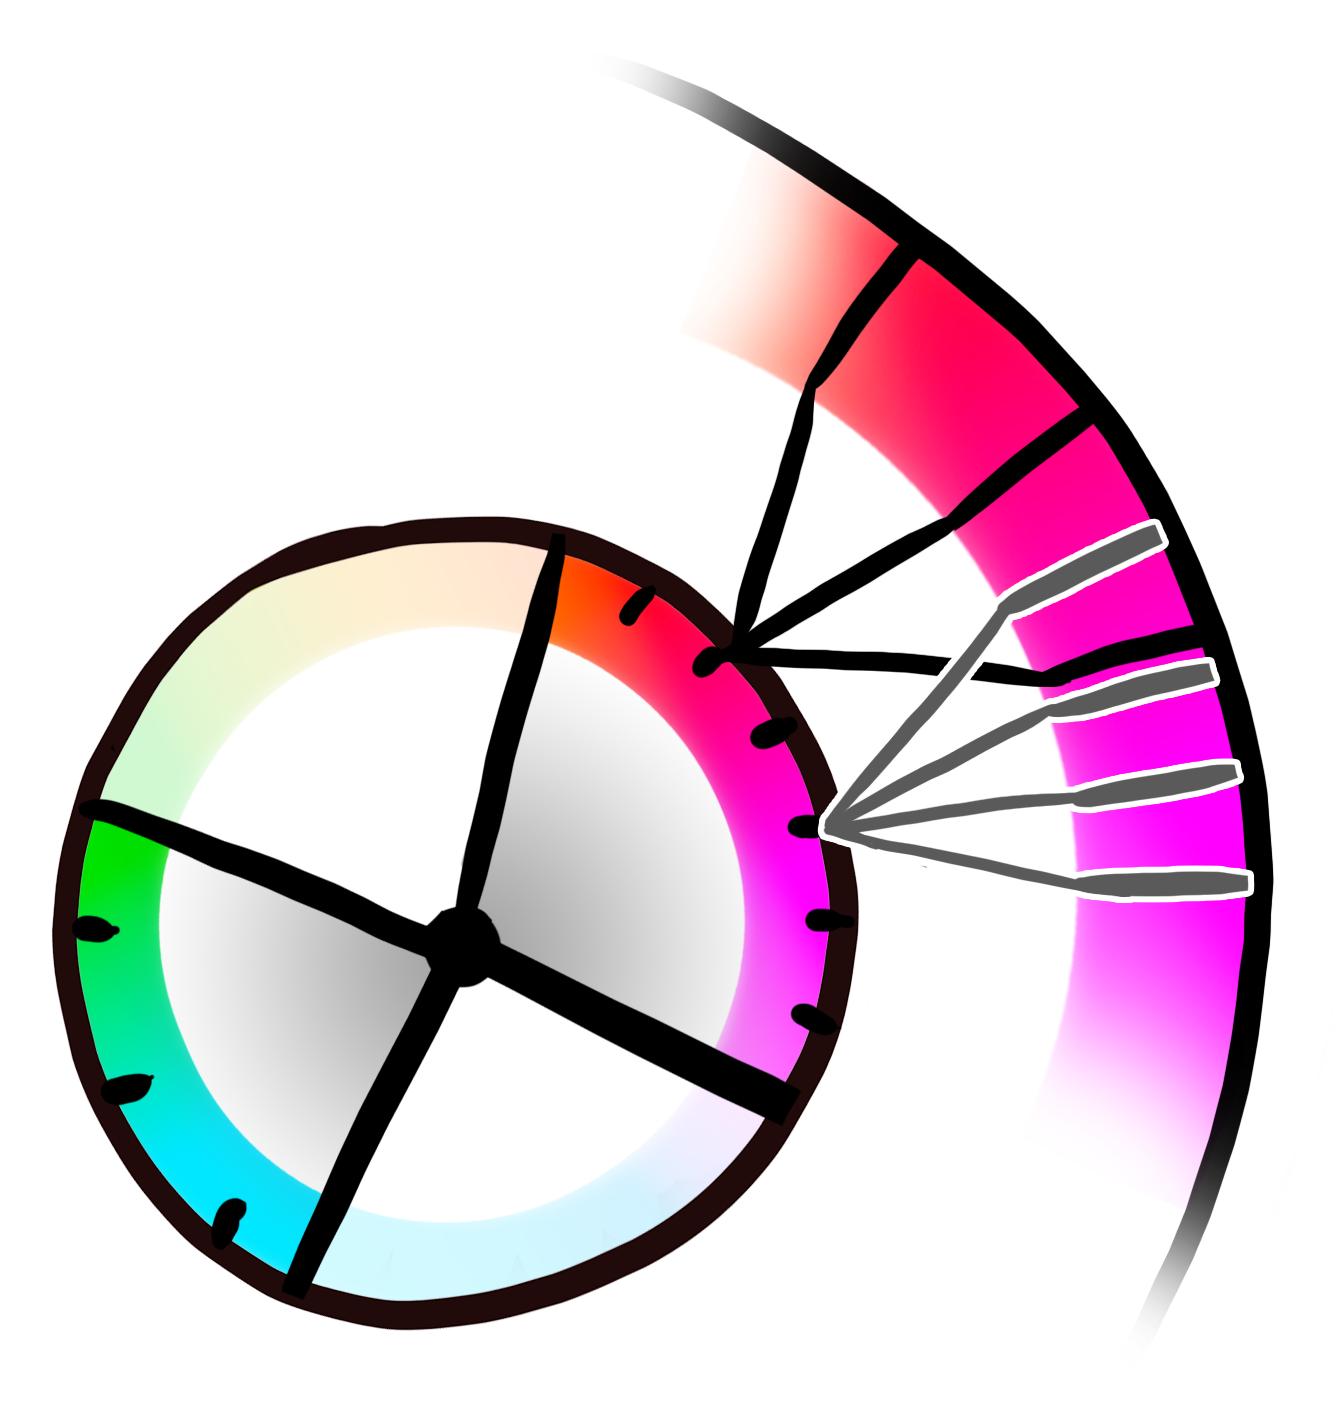
\includegraphics[width=0.4\linewidth]{Figures/overlap}
		\caption{The hierarchical color assignment for the protein chains. 
			The spacing between the protein domains (x,y,z) and (x',y',z',w') is predetermined based on the number of domains. 
			Unlike the tree-based coloring approach~\cite{tennekes2014tree} we allow colors to be reused across domains of different protein types (see 10 and 12) to offer more discriminability.
		}
		\label{fig:overlap}
	\end{figure}
	
		\begin{figure*}[t]
			\centering
			\includegraphics[width=1\linewidth]{Figures/results_4}
			\caption{Various snapshots from the Chameleon system.
				As the camera position changes, the discriminability between protein types is optimized.
				The color palette widget at the bottom left allows us to visualize the distribution of the groups along the hue circle.}
			\label{fig:results_1}
		\end{figure*}
		
		\begin{figure*}[t]
			\centering
			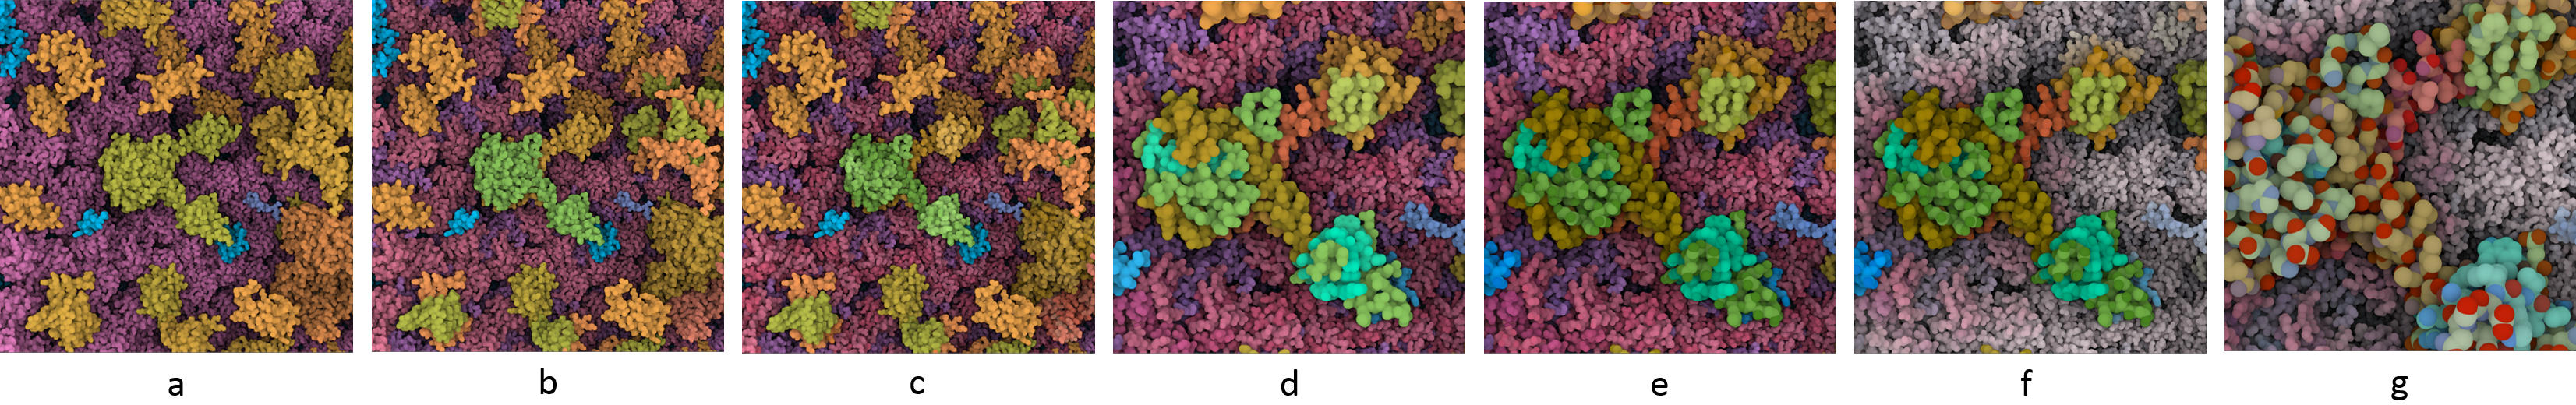
\includegraphics[width=1\linewidth]{Figures/results}
			\caption{The hue, chroma, luminance modulation in sequential steps.
				(a) only the protein colors are show, (b) protein domains are show via hue modulation, (c) secondary structures are shown via luminance modulation, (d) secondary structures are shown via hue modulation
				(e) atom types are shown via luminance modulation, (f) focus is highlighted via chroma modulation, (g) atom types are shown via hue modulation}
			\label{fig:results_2}
		\end{figure*}
	
	
	
	\begin{figure}
		\centering
		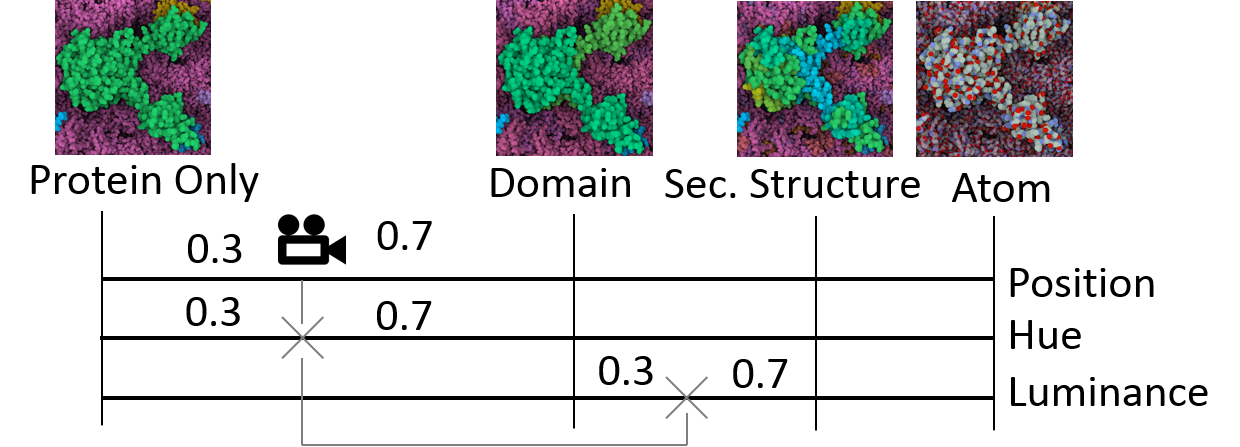
\includegraphics[width=1\linewidth]{Figures/zoomfigure}
		\caption{Interpolation of hue and luminance depends on the position of the view. The black camera in the top line shows the position of the viewer with respect to the different levels. The grey crosses show the corresponding positions for interpolating hue and luminance.
			The hue is equal to a linear interpolation of the two neighbouring levels shown in the middle line, here compartment and protein. Luminance is equal to a linear interpoation of the next two levels, here protein and domain, visible on the bottom line. The interpolation is based on the ratio of the distance to the neighbouring levels, here 0.3 and 0.7. }
		\label{fig:zoom_continuum}
	\end{figure}
	
	
	\section{Context Desaturation}
	\label{sec:chroma}
	
	%	\textbf{MWa rewrite BEGIN}
	
	Due to our hierarchical color assignment, domain colors of neighboring proteins or secondary structures of neighboring domains may be assigned identical colors, see Figure~\ref{fig:overlap}.
	To increase color discriminability, and reduce occurrence of similar colors, we modulate the chroma to generate a focus+context effect. 
	We select the protein with the highest screen coverage in the central region of the screen as focus element.
	Based on the size of the protein and its location we define a spherical region in 3D which constitute the focus region.
	Outside this region, we progressively decrease the chroma value as we zoom in the focused protein, to ensure optimal color discriminability of the focus protein's colors with respect to all other colors in the scene. 
	The zoom levels distances between which the desaturation effect begins and ends are arbitrarily defined.
	Should the focused protein change abruptly, we interpolate the focus region centroid and radius between the previously and currently focused protein to avoid flickering artifacts.
	%	Figure \ref{fig:focusContext} shows a single focus protein with XX domains. 
	
	%	\textbf{Just to be sure: this does not solve the problem of similar colors of secondary structures of different domains on the same protein?}
	
	%	\textbf{MWa rewrite END -- remove next 2 paragraphs in case of acceptance}
	
	%	The colors of the lower hierarchy-levels (chains, secondary structures) are chosen hierarchically, based on the color of their parent in the previous level.
	%	For example, the hue value of a chain is sampled around the hue of its protein, with an arbitrarily defined offset, see Figure~\ref{fig:coloroverview}.
	%	Our system provide optimal hue distribution of protein colors for proteins based on the visibility information, which guarantees that protein will always be assigned unique and distinct colors.
	%	However, this is not the case for following levels of the hierarchy, where chains colors are likely to overlap with those of neighbouring proteins.  
	%	This limitation is principally caused by the significant discrepancies between the different levels.
	%	Indeed between single proteins and protein domains the difference in term of size is much smaller than between compartments and proteins, see Figure~\ref{fig:Picture2}.
	%	Given such constraint, we must rapidly ensure that the color information for the next level will be available, which cannot easily be achieved based-on visibility and without dramatically reshuffling the colors.
	%	
	%	Therefore we rely on a focus+context approach instead, to optimize the view and guaranty a minimum degree or repeated colors.
	%	Indeed, when closely observing protein properties, it is very unlikely that the viewer will also observe properties of all the surrounding proteins, as commodity hardware does not offer enough pixels to render all the context proteins with enough details to be relevant to the viewer.
	%	Therefore we define a focus region outside which the colors of the proteins will be desaturated to reduce occurrence of colors used in focus region.
	
%	\begin{figure}		
%		\centering
%		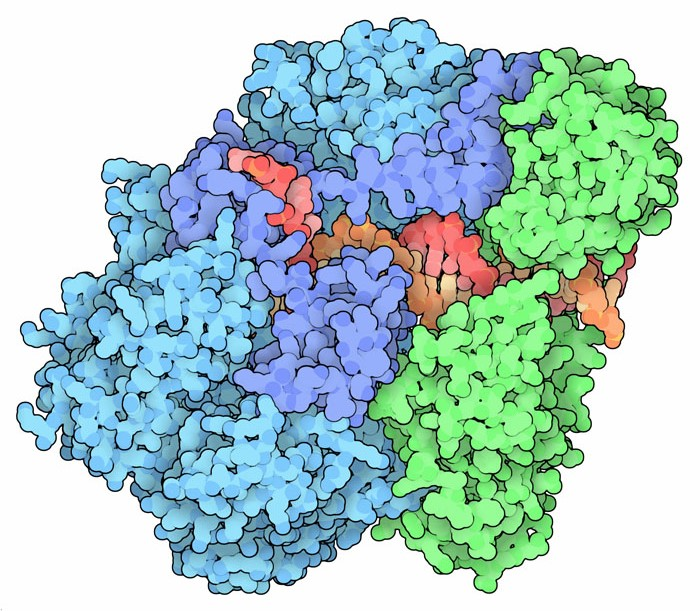
\includegraphics[width=0.5\linewidth]{Figures/goodsell_protein}
%		\caption{An illustration of a protein using a popular color scheme from David Goodsell. The hue is used to discriminate between the protein domains, while the luminance is used to differentiate carbon atoms from the rest.}
%		\label{fig:goodsell_protein}
%	\end{figure}
	
	
	
	
	
	\section{Luminance Modulation}
	\label{sec:luminance}
	
	So far, we used the hue channel to discriminate structures on different zoom levels and the chroma to distinguish focus proteins from the context. 
	The final color channel we can manipulate is luminance. 
	Illustrators sometimes use the luminance channel to indicate structural properties in lower hierarchy levels, as shown in Figure \ref{fig:motivation}. 
	This is a reasonable choice, given that hue is known to be an effective channel to encode low-frequency information, while luminance is more effective to encode high-frequency information~\cite{bergman1995rule}. 
	
	%	\textbf{Figure goodsell layer by goodsell himself}
	
	For each hierarchy level, we therefore not only assign unique hues, but also unique luminance values. 
	We modulate the pre-defined luminance value by a small range to avoid extensive visual clutter. 
%	In the example of Figure \ref{fig:zoomLevels}, we use a luminance range of 20 to distinguish the sub-elements. 
	Thus, this luminance modulation does not help to clearly discriminate or identify structures on a lower hierarchy level, but it is a subtle indication of lower-level structural properties. 
	
	Like the hue, the luminance value is defined by the distance of the camera to the respective structures. 
	Given pre-defined distances for distinct hierarchy levels, the colors are interpolated linearly between two neighboring levels. 
	However, unlike the hue, we do not interpolate between the actual hierarchy levels, but interpolate between the next two hierarchy levels with the current interpolation factor instead, as illustrated in Figure \ref{fig:zoom_continuum}. 
	This way, the hue and the luminance encode different hierarchy levels, yet both color channels are seamlessly interpolated for smooth transitions. 
				
	
	
		
	\section{Results}
	\label{sec:results}
	
	To showcase the capabilities of the Chameleon, we applied it to a mesoscale molecular scene. 
	The dataset was provided by the domain experts and modeled with cellPACK \cite{johnson2015cellpack}, a tool for procedural generation of large biomolecular structures.
	cellPACK summarizes and incorporates the most recent knowledge obtained from structural biology and system biology to generate comprehensive mesoscale models. 
	Based on experimentally obtained data (e.g. data such as protein structure, concentration and spatial distribution), the tool is able to generate entire models of viruses and cells via a packing method based on collisions constraints.
	We use cellVIEW \cite{muzic2015cellview} for the rendering part, which is a tool designed to efficiently render large molecular scenes on the GPU and is implemented in Unity3D. \\
	
	The dataset which we showcase is a model of an HIV particle in blood serum which contains 20502 instances of 46 different protein types including two lipid membrane layers.
	The protein types are grouped together based on their location.
	There are 6 different protein groups in the dataset; the blood plasma proteins (18 types), the lipids (2 types), the envelope surface (5 types) and interior proteins (15 types), the capsid surface (1 type) and interior proteins (5 types).
	Figure \ref{teaserImage} shows progressive zooming from the entire virus to single atoms.	
	Initially the blood plasma proteins in green, and the matrix protein in purple, dominate the color palette simply because they have more protein types than other compartments, like the capsid proteins in orange.	
	As we get closer to the capsid proteins in orange, we can observe that the colors become more distinguishable.	
	To visualize the results of the view-dependent color palette optimization more precisely, we also developed a custom palette widget, results are show in Figure~\ref{fig:results_1}.
	Figure~\ref{fig:results_2} shows all the sequential steps we take to progressively reveal the protein properties as we zoom in.\\
	%The second dataset, shown in Figure \ref{fig:nofig} is a model of an immature HIV which contains 1081 instances of 13 different protein types, and one bi-lipid membrane. \\
	
	The Chameleon relies on GPU computing to provide a smooth and responsive user experience.
	Since we perform the all the coloring operations in post-processing, the size of the dataset has only little impact on the performance. 
	We benchmarked the computation speed at HD resolution (1920$\times$1080) on a machine equipped with an Intel Core i7-3930 CPU 3.20 GHz machine coupled with a GeForce GTX Titan X graphics card with 12GB of video RAM.
	We measured \textbf{0.5 ms} on average to count the visible instances when zooming out on the entire dataset, which in the most extreme case since a very large number of proteins are visible.	
	It took \textbf{1.2 ms} to compute the screen pixel coverage of the protein types with the same configuration.
	The last stage of the pipeline in which we assign the final hue, chroma, and saturation values to each pixel took \textbf{1.3 ms} on average, this also includes the cost of reading back the visibility information to the CPU for the force-based hue assignment.
		
	%\section{Technique (section written by Nicholas)}
	%
	%When applying a coloring scheme to data of this type, several things need to be taken into account. 
	%First, the representation should support the level the user is looking at, e.g. not show the protein domains when the user is looking at the compartment level. 
	%Second, switching from one level to another should not be confusing.
	%Third, the user should be able to easily identify useful information at the level he is looking at. 
	%Because predetermining all the colors for each item in the scene and not allowing for view dependency will, with enough data, guarantee that data points will become indistinguishable. 
	%Fourth, the coloring must allow the user remain orientated and determine what belongs to the stuff he is interested in. 
	%For example, he needs to know where a compartment ends and the next one begins.
	%Stress the fact that temporal coherence and discriminability by color are contradicting each other if we need a lot of colors (give numbers for HIV!). 
	%Ware (?) points out that luminance is more useful for encoding high-frequency information, while hue is easier to interpret for encoding low-frequency information. 
	%
	%This is also reflected in the well-known ColorBrewer color schemes, where colors of categorical palettes differ primarily by hue, while quantitative color schemes operate mostly on luminance level.  
	%We therefore use utilize the HCL color space that separates these two properties into different dimensions (luminance is the vertical axis, while hue and chroma are represented on the perpendicular planes as polar coordinates). 
	%Another useful aspect of the HCL color space is that it is simply an alternative representation of the CIEL*a*b* color space and therefore perceptually linear. 
	%This means that we can linearly link changes in the color space to perceptual responses. 
	%We start by assigning each item on the lowest LOD a distinct hue. 
	%Since the lowest hierarchy level comprises the entire model, this assignment is static and does not change with the viewing angle. 
	%Given the number of elements $n$ on the lowest LOD, the desired luminance and chroma, the hue of the i’th element is simply defined by $h_i=i*360/n$. 
	%This results in $n$ isoluminant colors with equidistant hues. 
	%(Chroma is luminance-depending if we consider the sRGB boundaries, but we don’t do this now!)
	%We use a hue circle here, but any parametric curve within the HCL space could be used. 
	%In this case, the colors would not be isoluminant, but still equidistant in the perceptually linear color space. 
	%Each section applies force on its neighbouring section, proportional to the number of different kinds of proteins that are visible. 
	%This means that the section can grow and shrink, depending on visibility. If a compartment is not visible, then the section shrinks to a size zero. 
	%
	%However, a degree of consistency is still desired. It would be unwanted for a compartment to switch over to the opposite color, such as blue to yellow.  
	%As such something needs to be in place to keep compartments from moving too far.
	%The switch to the proteins color occurs when the distance is greater than 5*2.3 =5*jnd in cielab space [Mahy 94 evaluation after adoption]. 
	%This is equal to an angle of X on the hue circle.
	%
	%Another problem is how do we choose the colors for the domains? Their color needs to be view dependent as well as near to the color of the protein they belong to. 
	%The color of the chains does not Interact with the color of the other proteins, but does if they are showing their chains. 
	%Whether or not the chains are shown depends on the how close the camera is to the protein, unless the color distance would be below a certain amount (5*2.3) (8.8 degrees). 
	%The hue circle is reused to show the colors of the chains. See fig[]. 
	%The chains don’t cause any force on the proteins, and the proteins cause no force on the chains. 
	%The chains of two different proteins can cause force on one another if they are being shown. 
	%Because the chains would normally surround the entire circle, they only push each other away to a maximum distance of X. 
	%This allows for the chains to have similar colors to the proteins.
	
	\section{User Study}
	\label{sec:study}
	We conducted a user study with domain experts in biology in order to evaluate our visualization and to improve it based on the feedback.
	We wanted to know whether the colors helped to solve the tasks.
	Furthermore, we wanted to know how disruptive the changing colors are, so we did not inform the users about their dynamic behaviour. 
	Instead, we tested whether they would notice the change.
	The user study was conducted in two study runs. 
	In the first run, two domain experts tested the software. 
	Their feedback was used to adapt the software, which was then tested by five domain experts.
	
	%In the first iteration the secondary structures were identifiable through luminance, not color. They had the same hue as the domain they belonged to, simply lighter ($\beta$-sheets) or darker ($\alpha$-helices);
	
	\subsection{Users}
	We gathered 7 domain experts. 6 were PhDs. and PostDocs, and one was a master student. All users were experts in the field of molecular biology. 
	To conduct their research, the participants use visualizations on the protein or molecular level.
	
	
	\subsection{Study Design}
	We performed a qualitative study instead of a quantitative lab experiment.
	In a qualitative study, the user is given a visualization and is tasked with solving some questions. 
	In contrast to a quantitative user study, where task completion times and errors across multiple conditions are compared, the goal is to measure what the user can discover about the dataset.
	There are two reasons for this choice.
	First, the task is too complex to be captured well by these simple measurements. 
	Second, there is no established baseline condition.
	Without means to distinguish structures on different search levels, the task would not be solvable and therefore either create a bias towards our technique or not fully demonstrate its potential.\\
	The study consisted of two parts. In the first part the user was asked to identify structures on different levels. 
	It also allows us to measure what information can be found.  
	In the second part the users explored the HIV virus freely, and we observed what they discovered.
	
	\subsection{Structure Identification Task}
%	\begin{figure}
%		\centering
%		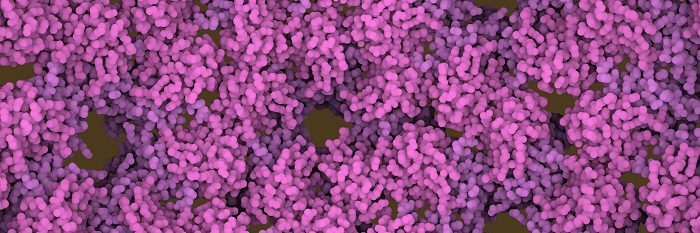
\includegraphics[width=1\linewidth]{Figures/pentamerStudy}
%		\caption{Rendering of Capsid during the second user study. In the center there is a pentamer, and to the left of it a hexamer.}
%		\label{fig:pentamerStudy}
%	\end{figure}
	Based on a description designed by a molecular bioligist and an illustrator, the first task was to investigate the capsid of the HIV. 
	The following is a shortened version of the description: \\
	
	\textit{
		The capsid encloses the genome (2 strands of RNA) along with different viral proteins. 
		The capsid protein is able to form hexamers and pentamers by shifting slightly in structure, and folds to form two domains connected by a flexible linker: the N-terminal domain and C-terminal domain. 
		The N-terminal domain is involved in forming the hexamers or pentamers, and the C-terminal domain is involved in dimer contacts between hexamers / pentamers. 
		There are two $\alpha$-helices in the N-terminal that stabilize the hexamers and pentamers. 
		As HIV is budding from an infected cell, the cellular enzyme cyclophilin A binds to the capsid. 
		On the surface of the capsid protein there is a loop with several proline amino acids, which is the bonding of cyclophilin.}\\
	
	The task which we gave to the users was to locate the following elements:
	
	\begin{enumerate}
		\itemsep0em 
		\item Capsid pentamer.
		\item N-terminal and C-terminal domain of capsid protein.
		\item Alpha helix in the N-terminal domain stabilizing the hexamers and pentamers.
		\item Binding site of cyclophilin A.
		\item Methionine amino acid within the alpha helix.
	\end{enumerate}
	
	Each structure was located on a different scale. 
	In the last task they were asked to find a Methionine amino acid molecule, for which they were given the chemical formula and a structural description.
	The task of finding the pentamer was added so the users would practice moving the camera around. 
	Pentamers and Hexamers share the same structure, they simply have 5 or 6 capsid proteins respectively. 
	However, there are only 12 pentamers in the capsid.
	Therefore, recognizing a pentamer was easier than actually finding one, because their sparcity was the largest obstacle in finding them.
	
	All capsid proteins, i.e., both hexamers and pentamers had the same color at the protein level. They could be distinguished only by shape. By zooming to the domain level, the N- and C-terminals are assigned different colors. At the secondary structure level, $\alpha$-helices and $\beta$-sheets received different colors. In the first study run, the helices had lower luminance than the domain they belonged to, and the sheets had higher luminance. In the second study run, each secondary structure received its own color. 
	The cyclophiline binding site was not part of an $\alpha$-helix or $\beta$-sheet.
	This was to test whether or not the user could find a structure that was not explicitly marked. 
	We did not show the amino acid level.
	To find the Methionine amino acid, the user had to look for a sulfur atom; there was no other amino acid with a sulfur atom near it, though there is a second one in the protein. 
	If the user did not find the amino acid or realize that they needed to look for a sulfur atom, they were asked to find a sulfur atom instead.
	
	
	
	
	
	\subsection{Free Exploration}
	In the structure identification task, we were interested in whether or not users could complete the tasks, as well as reasons for potential failures. 
	In the exploration part, users could freely navigate through the visualization while thinking aloud. We were interested in the insights users would gain while exploring the model.
	Most important is the degree of exploration, as well as what the users were capable of finding or looking at, as the users were capable of focusing on many different objects as well as on different levels.
	
	\subsection{Results of First Study Run}
	\begin{table}
		
		\centering
		\begin{tabular}{| c | c | c |}
			\hline
			Task \textbackslash User & 1 & 2  \\
			\hline
			Pentamer       & n & n \\
			\hline
			C-terminal     & y & y \\
			\hline
			N-terminal     & y & y \\
			\hline
			$\alpha$-helix & n & y \\
			\hline
			Binding site   & y & y\\
			\hline
			Methionine      & partially & y \\
			\hline
		\end{tabular}
		
		\caption{Results of Task One in First Study Run}
		\label{table:tableIterationOne}		
	\end{table}
	
	
	Two users participated in the first study run. 
	Their results can be seen in Table~\ref{table:tableIterationOne}.
	In the first task neither found the pentamer. 
	Both found the N and C terminals. 
	Both found the Cyclophilin binding site. 
	Only one found the alpha helix and the amino acid, while the other found a different sulfur atom.
	
	In task 2 neither user interacted significantly with the visualization. This was likely due camera control issues. 
	One of the participants had trouble getting the camera to point where he wanted in general, the other at the lower levels.
	This is partially due to the method of control over the camera. 
	The controls allowed panning, zooming and rotating the camera. 
	Furthermore, the movement of the camera did not take the semantic or zoom level into account.
	
	\subsection{Feedback}
	Two issues were identified in the first study run. 
	The first problem was camera control. 
	In order to use the camera when zoomed further in a certain degree of experience was required, otherwise the camera could easily be moved too far.
	In order to fix this, we altered the camera controls so the user could slow down the camera movement significantly.
	
	The other issue was the detection of the secondary structures. 
	One of the users could not detect the $\alpha$-helices. The other could, but did not use the coloring of the secondary structure.
	Instead, he looked at the correct area on the atomic level and found it based on the atomic structure.
	We noticed that there were several helices and sheets in the protein. 
	This meant that the altering of the luminance might not seperate a helix from the surrounding area. 
	Therefore, we altered the coloring of the secondary structures to be based on hue, and each secondary structure would receive its own hue.
	This coloring is based on the same principle as other levels.
	
	
	\subsection{Results of Identification Task Second Study Run}
	In the second study run, none of the users had significant issues with the camera, though some controlled it better than others.
	For the 5 users, as shown in Table~\ref{table:seconrund}, the results are as follows:
	\begin{table}
		
		\centering
		\begin{tabular}{| c | c | c | c | c | c |}
			\hline
			Task \textbackslash User & 1 & 2 & 3 & 4 & 5 \\
			\hline
			Pentamer       & y & y & n & y & y\\
			\hline
			C-terminal     & y & y & n & y & y \\
			\hline
			N-terminal     & y & y & n & y & y  \\
			\hline
			$\alpha$-helix & y & y & n & y & y \\
			\hline
			Binding site   & y & y & y & y & y \\
			\hline
			Methionine      & y & partially & n & partially & n  \\
			\hline
		\end{tabular}
		\caption{Results of Task One in Second Study Run}
		\label{table:seconrund}
	\end{table}
	Apart from user 3, users could identify structures across all levels fairly well. 
	Users 2 and 4 found a Methionine, but not the correct one. 
	This is because they didn't notice the colors, so they didn't know exactly where to restrict their search.
	Therefore, they found one of the other Methionine amino acids in the protein.
	
	
	\subsection{Observations}
	One of the users failed to identify the pentamer and mixed up the N and C terminals. 
	In the capsid, there is some space between the hexamers. 
	From the users description of the pentamer and of the capsid structure, he mixed up the interior and exterior of the hexamers. 
	The user who considered a subset of the C-terminal as the entire domain had zoomed past the domain level to the secondary structure level.
	The user in the second study run who did not find the $alpha$-helix also did not find a sulfur atom. He never zoomed in closely enough to the proteins to change the colors to the atom colors. It is likely that he became discouraged due to his failure to find the helix, as well as believing there was no way to identify the sulfur atom.
	
	With the exception of one user, the only problems with identifying structures came at the secondary structure and amino acid level. 
	The amino acid level was significantly more difficult, as the amino acids were not explicitly visually represented. 
	The users had to find it based on one atom, a strategy which they had to arrive at themselves. 
	
	
	
	\subsection{Results of Exploration Task Second Study Run}
	
	The actions of the users in the second task were extremely varied. 
	Unlike the first study run, 4 of the 5 users spent time exploring the virus. 
	However, the parts they explored varied significantly. 
	
	User 1 looked at the membrane and the proteins in the matrix. 
	He found one of the capsid hexamers that can also be found in the matrix.
	User 2 tried to find the other amino acids in the helix that had been mentioned in the description. 
	He also took particular interest in the Cyclophilin binding site. 
	He looked at its structure and identified several of the amino acids.
	The third user, who had significant issues finding the structures, did not explore the HIV significantly.
	The fourth user looked at the atomic structure of proteins that were not part of the capsid.
	However he did not explore any protein in detail. 
	Instead, he was more interested in the variety of proteins in the HIV.
	The last user took interest in the membrane and the proteins near it.
	He was interested in the structure of the protein and in the area where it met the membrane.
	Of those who explored the virus, the users spent just short of 10 minutes on average for exploration.
	
	
	
	
	\subsection{Feedback}
	An interesting aspect was how little the users noticed the changing colors, yet still used the colors to identify the areas.
	When asked about the changing colors in the post-experiment interview, all users noticed the changing colors when zooming to the atomic level, but only one noticed it on all levels, while a second thought something odd was occuring on the secondary structure level. 
	
	Still, every user that found the N and C terminals referred to them by their color. 
	Several referred to alpha helices by color. 
	This means that the visualization succeeded in creating a smooth transition between the levels, and was still useful, despite the users not being aware of its support. 
	Furthermore, the fact that most students were succesful at least up to the secondary structure level indicates that our multiscale visualization technique can be used on each level. 
	Overall, users liked the study and visualization, but thought the tasks were very difficult.
	
	
	The largest difference between the study runs was the degree of exploration in the second task. In the first task, neither user explored the HIV extensively. In contrast, the users from the second study run explored the virus on different levels and areas. Likely this was affected significantly by the degree of control over the movement through the visualization. In the first study run, the users had significant control issues which were absent in the second study due to changes. In both study runs no users reported that they got lost or confused by the visualization.
	
	The users were also asked how useful they considered the visualization to be for their research, or what they could use it for. The users considered it useful for presenting their research and educating students, which is in line with our goal as mentioned in the beginning. However, only one user from the first study run considered it useful for his research. This is in a sense not surprising. Most users worked on the level of molecular structure or protein interactions. Furthermore, while it may be possible to visualize an entire virus, a physical simulation of one is a different problem. 
	
	
	Several users expressed a desire for alternative representations that they were more familiar with, such as cartoon representation for secondary structures.
	
	
	
	
	
	
	%\subsection{feedback to implement into method}
	
	
	%\subsection{stuff they'd like to see}
	%- obviously they'd like everything.
	%- cartoon representation
	%- polarity etc.
	
	
	%\subsection{uses and applications}
	%
	%
	%We opted to perform a qualitative evaluation with XX biologists consisting of two blocks.
	%In the first block, users had to identify a set of pre-defined structures across multiple levels of scale in the HIV model. 
	%In the second block, users could freely explore the scene.
	%In both blocks, users were encouraged to “think aloud”. 
	%Sessions were observed by one to two study administrators, the screen was captured, and audio was recorded. 
	%The session was concluded by a questionnaire and an audio-recorded semi-structured interview. 
	%The task was provided by a professor of molecular biology and well-known illustrator of biological models. 
	%Users were first provided by a description of the HIV capsid protein, which is the single protein building up the HIV capsid.
	%Then they were asked to identify structures from this description in the HIV visualization, namely the capsid compartment itself, a special protein compound of the capsid, the two protein domains, secondary structures acting as binding sites, and a dedicated amino acid. 
	%The study was conducted on a (laptop specification, screen, color calibration). 
	%Users were sitting approximately ... cm from the screen, but were free to move. 
	%Before performing the actual study task, users were demonstrated how to navigate in the scene, and how to switch on and off certain sub-compartments. 
	%This was necessary so that all items were accessible without occlusions. 
	%We decided to perform a qualitative evaluation as our visualization is new, and there is currently no visualization that allows the user to look at all levels in a similar manner, so we do not have a method of comparison.
	%Our goal primarily was to see whether domain experts can identify the individual structures, whether this would be possible without color coding at all, and whether the view-dependent color assignment was irritating for them. 
	%
	%Users
	%The users were molecular biology students. As such, they had some but limited knowledge of the field [tbd may be variation]. 
	%As such, there needed to be an explanation of what they were looking for. The students ranged from x to y years studying.
	%
	%Results
	%-	How many students found the different targets
	%-	Insights
	%-	Probably need table of different types of insights.
	%-	Insights per minute  (ipm)
	%-	Answer to the questions we pose (table?)
	%-	People used
	%-	Number of people used
	%-	Describe type of study
	%-	Describe what this kind of study is.
	%-	Reference other (similar) studies
	%-	Argue why 
	%o	No baseline
	%o	No quantifiability (x in y seconds)
	%o	Want to measure usability
	
		\begin{figure}
			\centering
			
\includegraphics[width=1\linewidth]{Figures/hivscale}
			\caption{Illustration of the scale of the size of different objects. Note that amino acids and atoms are almost the same size. This indicates that a user will be equally far from a molecule when he wants to see the amino acids or the atoms.}
			\label{fig:hivScale}
		\end{figure}
		
	\section{Limitations}
	There are still two basic limitations to our coloring scheme. 
	The first is information on two different levels that are very close to each other, for example the amino acids and atoms. 
	Amino acids vary significantly in size and complexity, however some consist out of just several carbon atoms with even less other atom types, except for hydrogen. 
	Serine for example has only of 4 carbon atoms. This means the user will be approximately as far away from a molecule when he wants to see the atoms or amino acid information. 
	So the semantic scales reside on the same metric scale.
	Our visualization strategy is designed for distinguishing structures where each semantic level is assigned a unique metric level.
	In other words, their semantic scales reside on the same metric level, as shown in Figure~\ref{fig:hivScale}.
	The second problem is the variety of information. 
	For example, due to polarity, the electric charge may vary across a molecule. 
	Another interesting aspect of a protein might be hydrophobicity.
	A researcher may want to specify what kind of information he can see. 
	This means there are several paths that can be taken when zooming in.
	
	Another problem is alternative representations, such as cartoon representations of the secondary structure of proteins. 
	Several users expressed a desire for alternative representations that they were more familiar with.
	However, there can be some difficulty when using them. The cartoon representation for example has a lot of area which can be seen through. 
	If two proteins are one behind the other, then they can be hard to tell apart.
	

	
	
	
	\section{Conclusion and Future Work}
	The work presented here is a method that is capable of rendering a cell-like structure on different levels in a coherent and cohesive manner using color. 
	The hierarchical structure of the coloring technique, along with the visibility based variation in color allows users to navigate and inspect parts of the visualization without getting disorientated, while being subtle.
	Altering the color based on semantic zooming changes the meaning of color coding.
	Instead of discriminability for any situation, semantic color changes allow structures to be clustered or seperated as necessary.
	This is achieved while maintaining the connection between structures on different levels in a logical manner via the hierarchical nature of the coloring.
	Furthermore the coloring scheme is capable of showing structures on each level in a visually distinct manner. 
	The user study performed with our research prototype shows that users can find information in an HIV dataset on each level. 
	
	
	
	
	
	
	
	%\subsection{future work}
	There are several points that can be addressed in the future. The most obvious is to overcome the two basic limitations mentioned above. 
	The users also expressed interest in interacting with the visualization. 
	Structures such as the capsid consist out of numerous proteins. 
	The users wanted to be able highlight individual proteins or sections. 
	It might also be possible to couple this action with alternative representations for proteins, such as the cartoon representation.
	Finally, camera control can be adapted to the visualization. 
	Currently, the camera is controlled simply by inputing the desired direction of movement. 
	Alternate controls, such as tying the camera to a protein or structure, could be added.
	This would allow the user easier inspection of proteins or protein structures by making it easier for him to rotate around or follow the surface of an object.
	
	
	
	%% if specified like this the section will be committed in review mode
	\acknowledgments{
		The authors wish to thank A, B, C. This work was supported in part by
		a grant from XYZ.}
	
	\bibliographystyle{abbrv}
	%%use following if all content of bibtex file should be shown
	%\no
	{}
	\bibliography{Chameleon}
\end{document}
